\chapter{\babTiga}
\label{bab:metode}
% Sumber rancangan: app/SPEC.md, kode app/backend/app dan app/frontend/src,
% dataset/raw/*/DATASHEET.md, serta hasil terukur di app/results/.

\section{Desain Penelitian}
\label{sec:desain-penelitian}

Penelitian ini menggunakan pendekatan rancang bangun dan evaluasi komparatif. Artefak utamanya adalah Takar, aplikasi web untuk menyimpan resep dan prosedur operasional standar (SOP), menghitung variasi pesanan, mencatat pemakaian bahan, serta memberi rekomendasi operasional. Unit evaluasi ditetapkan sesuai keputusan yang didukung: satu pesanan untuk penskalaan resep, satu kueri keranjang untuk pasangan menu, satu pasangan produk--outlet--hari untuk peramalan, satu bahan--hari untuk simulasi persediaan, satu seduhan untuk sistem pakar, dan satu pertanyaan untuk asisten lokal. Pemisahan unit ini mencegah metrik dari tugas yang berbeda diperlakukan sebagai ukuran keberhasilan yang sama.

Rancangan dibagi menjadi analisis kebutuhan, pembuatan basis pengetahuan resep, implementasi aplikasi, pengujian fungsional, evaluasi algoritma, dan validasi eksternal. Data IBM dan Maven dipakai untuk pengembangan karena katalog produknya dapat dipetakan ke resep, tetapi keduanya merupakan data sampel fiktif. Oleh karena itu, penelitian ini juga menguji metode pada transaksi toko roti-kafe Edinburgh, penjualan mesin kopi ihelon, data seduhan konsumen UC Davis, resep eksperimen Batali, serta menu minuman Starbucks. Hasil pada sumber eksternal tidak dianggap sebagai bukti bahwa kinerja pada suatu kedai di Indonesia akan sama.

Arahan awal pembimbing menyebut Laravel dengan \textit{Progressive Web App}. Sesuai keputusan pengembangan tanggal 30 September 2026, implementasi memakai FastAPI (Python) dan Vue.js sebagai web responsif. Python dipilih agar pemrosesan data, pelatihan model, dan layanan API berada dalam lingkungan yang sama. Perubahan teknologi ini tidak mengubah masalah operasional, isi resep dari arahan, atau kebutuhan pencatatan inventaris.

\section{Tahapan Penelitian}
\label{sec:tahapan}

Tahapan penelitian mengikuti siklus analisis, perancangan, implementasi, pengujian, dan perbaikan bertahap. \textit{Product backlog} diturunkan dari tiga kendala utama arahan pembimbing: perbedaan takaran antarbarista, pelatihan staf baru, dan stok yang terpisah dari produksi. Kebutuhan variasi pesanan menjadi modul kalkulator; kebutuhan latihan menjadi panduan seduh dan checklist; kebutuhan stok menjadi buku besar pergerakan bahan. Modul AI menambah dukungan keputusan pasangan menu, peramalan dan pemesanan ulang, koreksi seduh, serta tanya-jawab berbasis pengetahuan lokal. Setiap iterasi menghasilkan fungsi yang bisa diuji melalui API dan antarmuka.

Gambar~\ref{fig:tahapan-penelitian} menunjukkan bahwa temuan pengujian dikembalikan ke rancangan. Urutan tersebut penting karena resep dan satuan bahan harus benar sebelum hasil penskalaan dipakai untuk memotong stok atau mengubah ramalan produk menjadi kebutuhan bahan. Setiap berkas hasil evaluasi menyimpan parameter, cap waktu, serta identitas data sehingga hasil pada Bab~\ref{bab:hasil} dapat ditelusuri ke prosedur pembuatnya.

\begin{figure}[htbp]
\centering
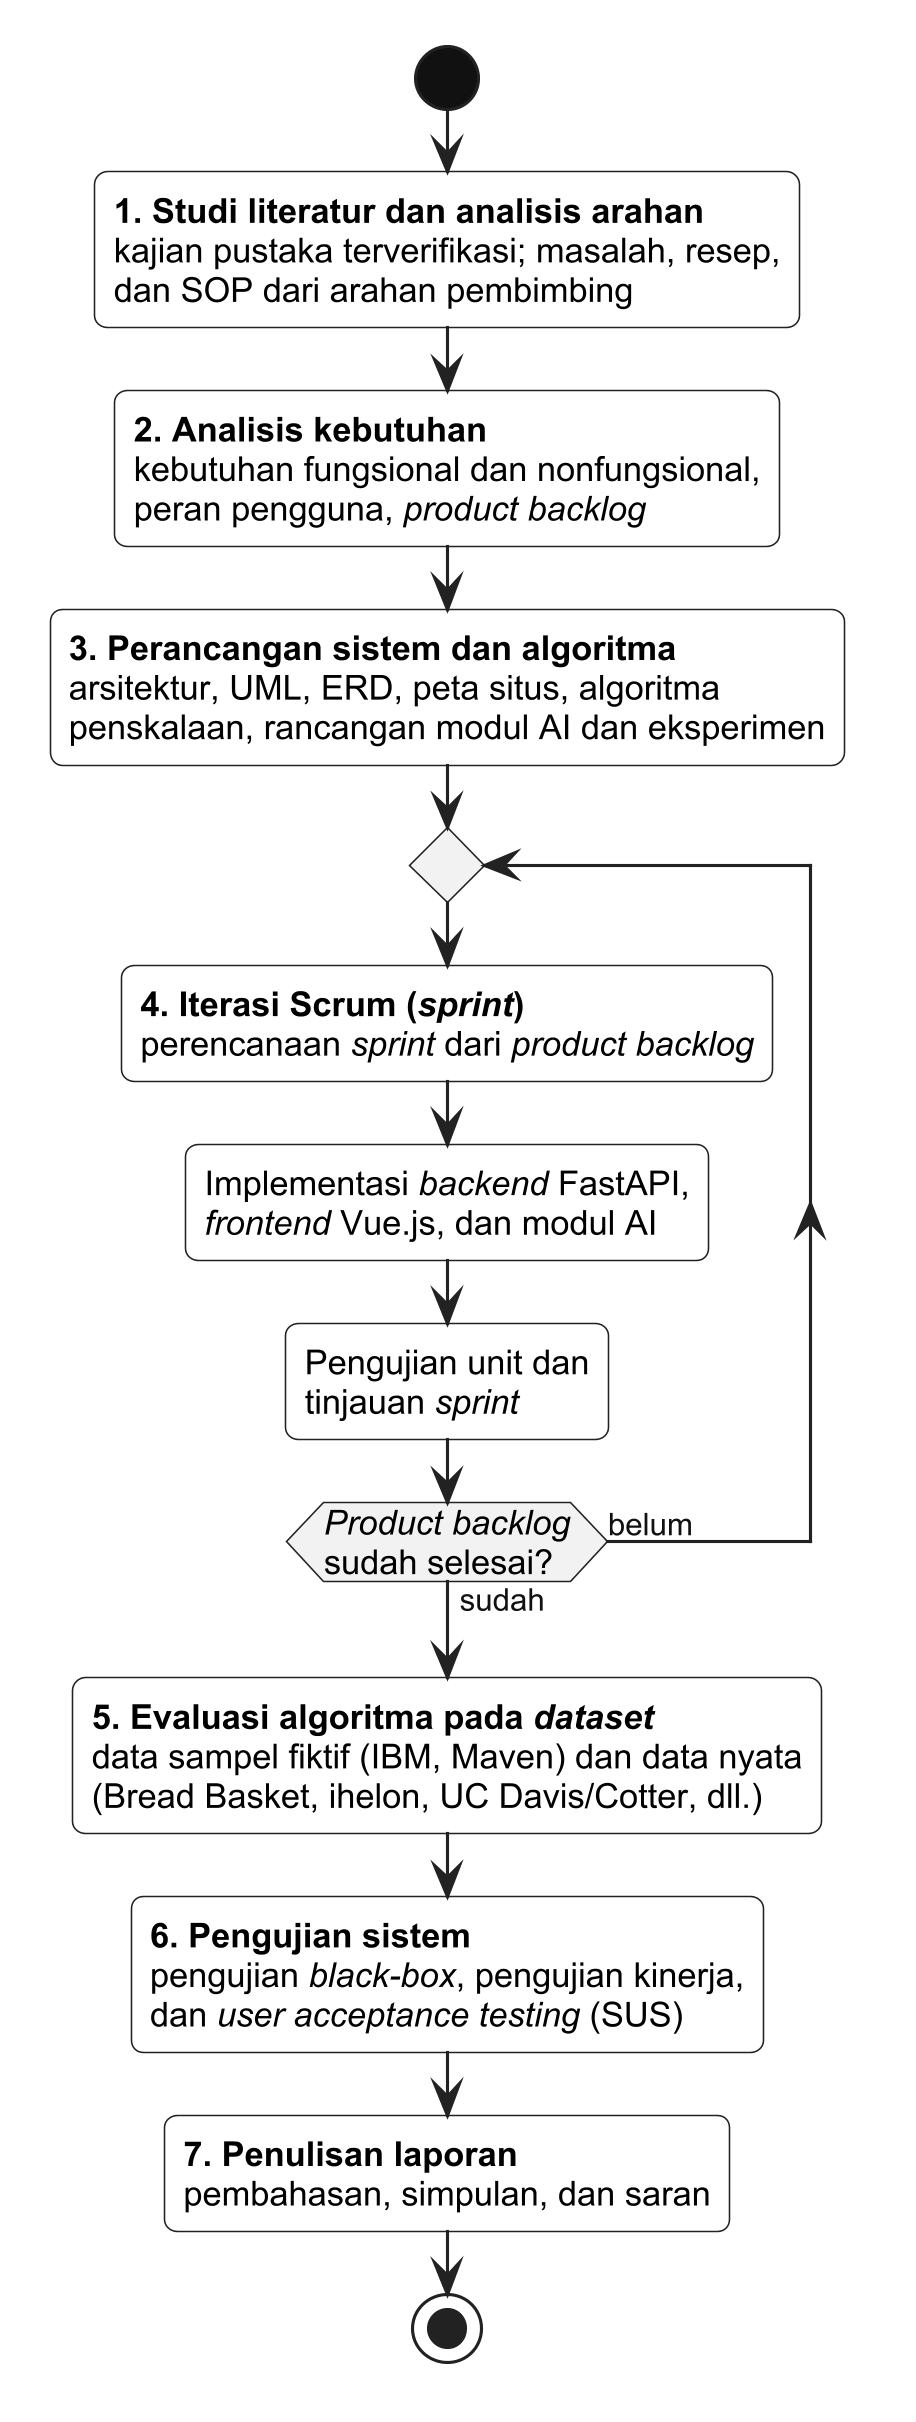
\includegraphics[width=.58\textwidth]{pic/tahapan_penelitian.png}
\caption{Tahapan Penelitian dan Umpan Balik Pengujian}
\label{fig:tahapan-penelitian}
\end{figure}

\section{Analisis Kebutuhan}
\label{sec:analisis-kebutuhan}

Pengguna dibagi menjadi manajer, kepala barista, dan barista. Ketiganya dapat melihat resep, SOP, kalkulator, panduan seduh, serta rekomendasi; dapat pula mencatat produksi dan mengerjakan checklist. Manajer dan kepala barista dapat mengubah resep, SOP, dan bahan serta mencatat penerimaan, penyesuaian, dan bahan terbuang. Hanya manajer dapat mengelola akun, menonaktifkan resep, dan melatih ulang model. Pemeriksaan hak akses dilakukan kembali di server, tidak hanya dengan menyembunyikan tombol di antarmuka.

Kebutuhan fungsional pertama adalah menyimpan resep dalam ukuran dasar beserta komponen, satuan, aturan penskalaan, parameter mutu, dan langkah pembuatan. Kebutuhan kedua adalah menghasilkan takaran per cangkir dan total pesanan untuk ukuran, jumlah cangkir, sajian panas atau dingin, tingkat manis, tambahan \textit{shot}, penggantian susu atau biji, dan dosis V60. Kebutuhan ketiga adalah menghubungkan produksi yang dicatat dengan pergerakan stok bahan secara atomik dan menjaga agar permintaan yang dikirim ulang tidak memotong stok dua kali. Kebutuhan keempat adalah menyajikan SOP, timer, ilustrasi tindakan yang mengikuti tahap resep, riwayat produksi, status bahan, dan penjelasan rekomendasi pada antarmuka berbahasa Indonesia. Saran pasangan menu yang memiliki padanan resep aktif harus dapat dibuka langsung sebagai panduan seduh.

Kebutuhan nonfungsional mencakup tampilan yang dapat digunakan pada tablet dan ponsel, validasi masukan di server, autentikasi JWT, kata sandi yang di-\textit{hash} dengan Argon2, pembatasan percobaan masuk, dan keluaran AI yang menyatakan sumber serta batasnya. Sistem ditujukan bagi satu outlet dengan basis data SQLite. Integrasi kasir, pesanan pembelian, multi-outlet, dan operasi luring berada di luar ruang lingkup. Angka stok awal, kemasan, harga, dan \textit{lead time} yang tidak tercantum dalam arahan adalah data contoh yang dicatat di \texttt{app/backend/app/seed/ASSUMPTIONS.md}.

\section{Perancangan Sistem}
\label{sec:perancangan-sistem}

Arsitektur pada Gambar~\ref{fig:arsitektur} memisahkan antarmuka Vue.js, API FastAPI, basis data SQLite, dan proses pelatihan atau evaluasi yang dijalankan sebagai skrip. Antarmuka mengirim permintaan JSON dengan token pengguna. API menerapkan autentikasi, validasi, logika resep dan stok, lalu membaca hasil model yang telah disimpan. Proses eksperimen membaca berkas data mentah dan menulis hasil JSON/CSV ke direktori \texttt{app/results}; berkas hasil tidak diisi manual. Pada mode satu port, FastAPI juga menyajikan hasil \textit{build} antarmuka.

\begin{figure}[htbp]
\centering
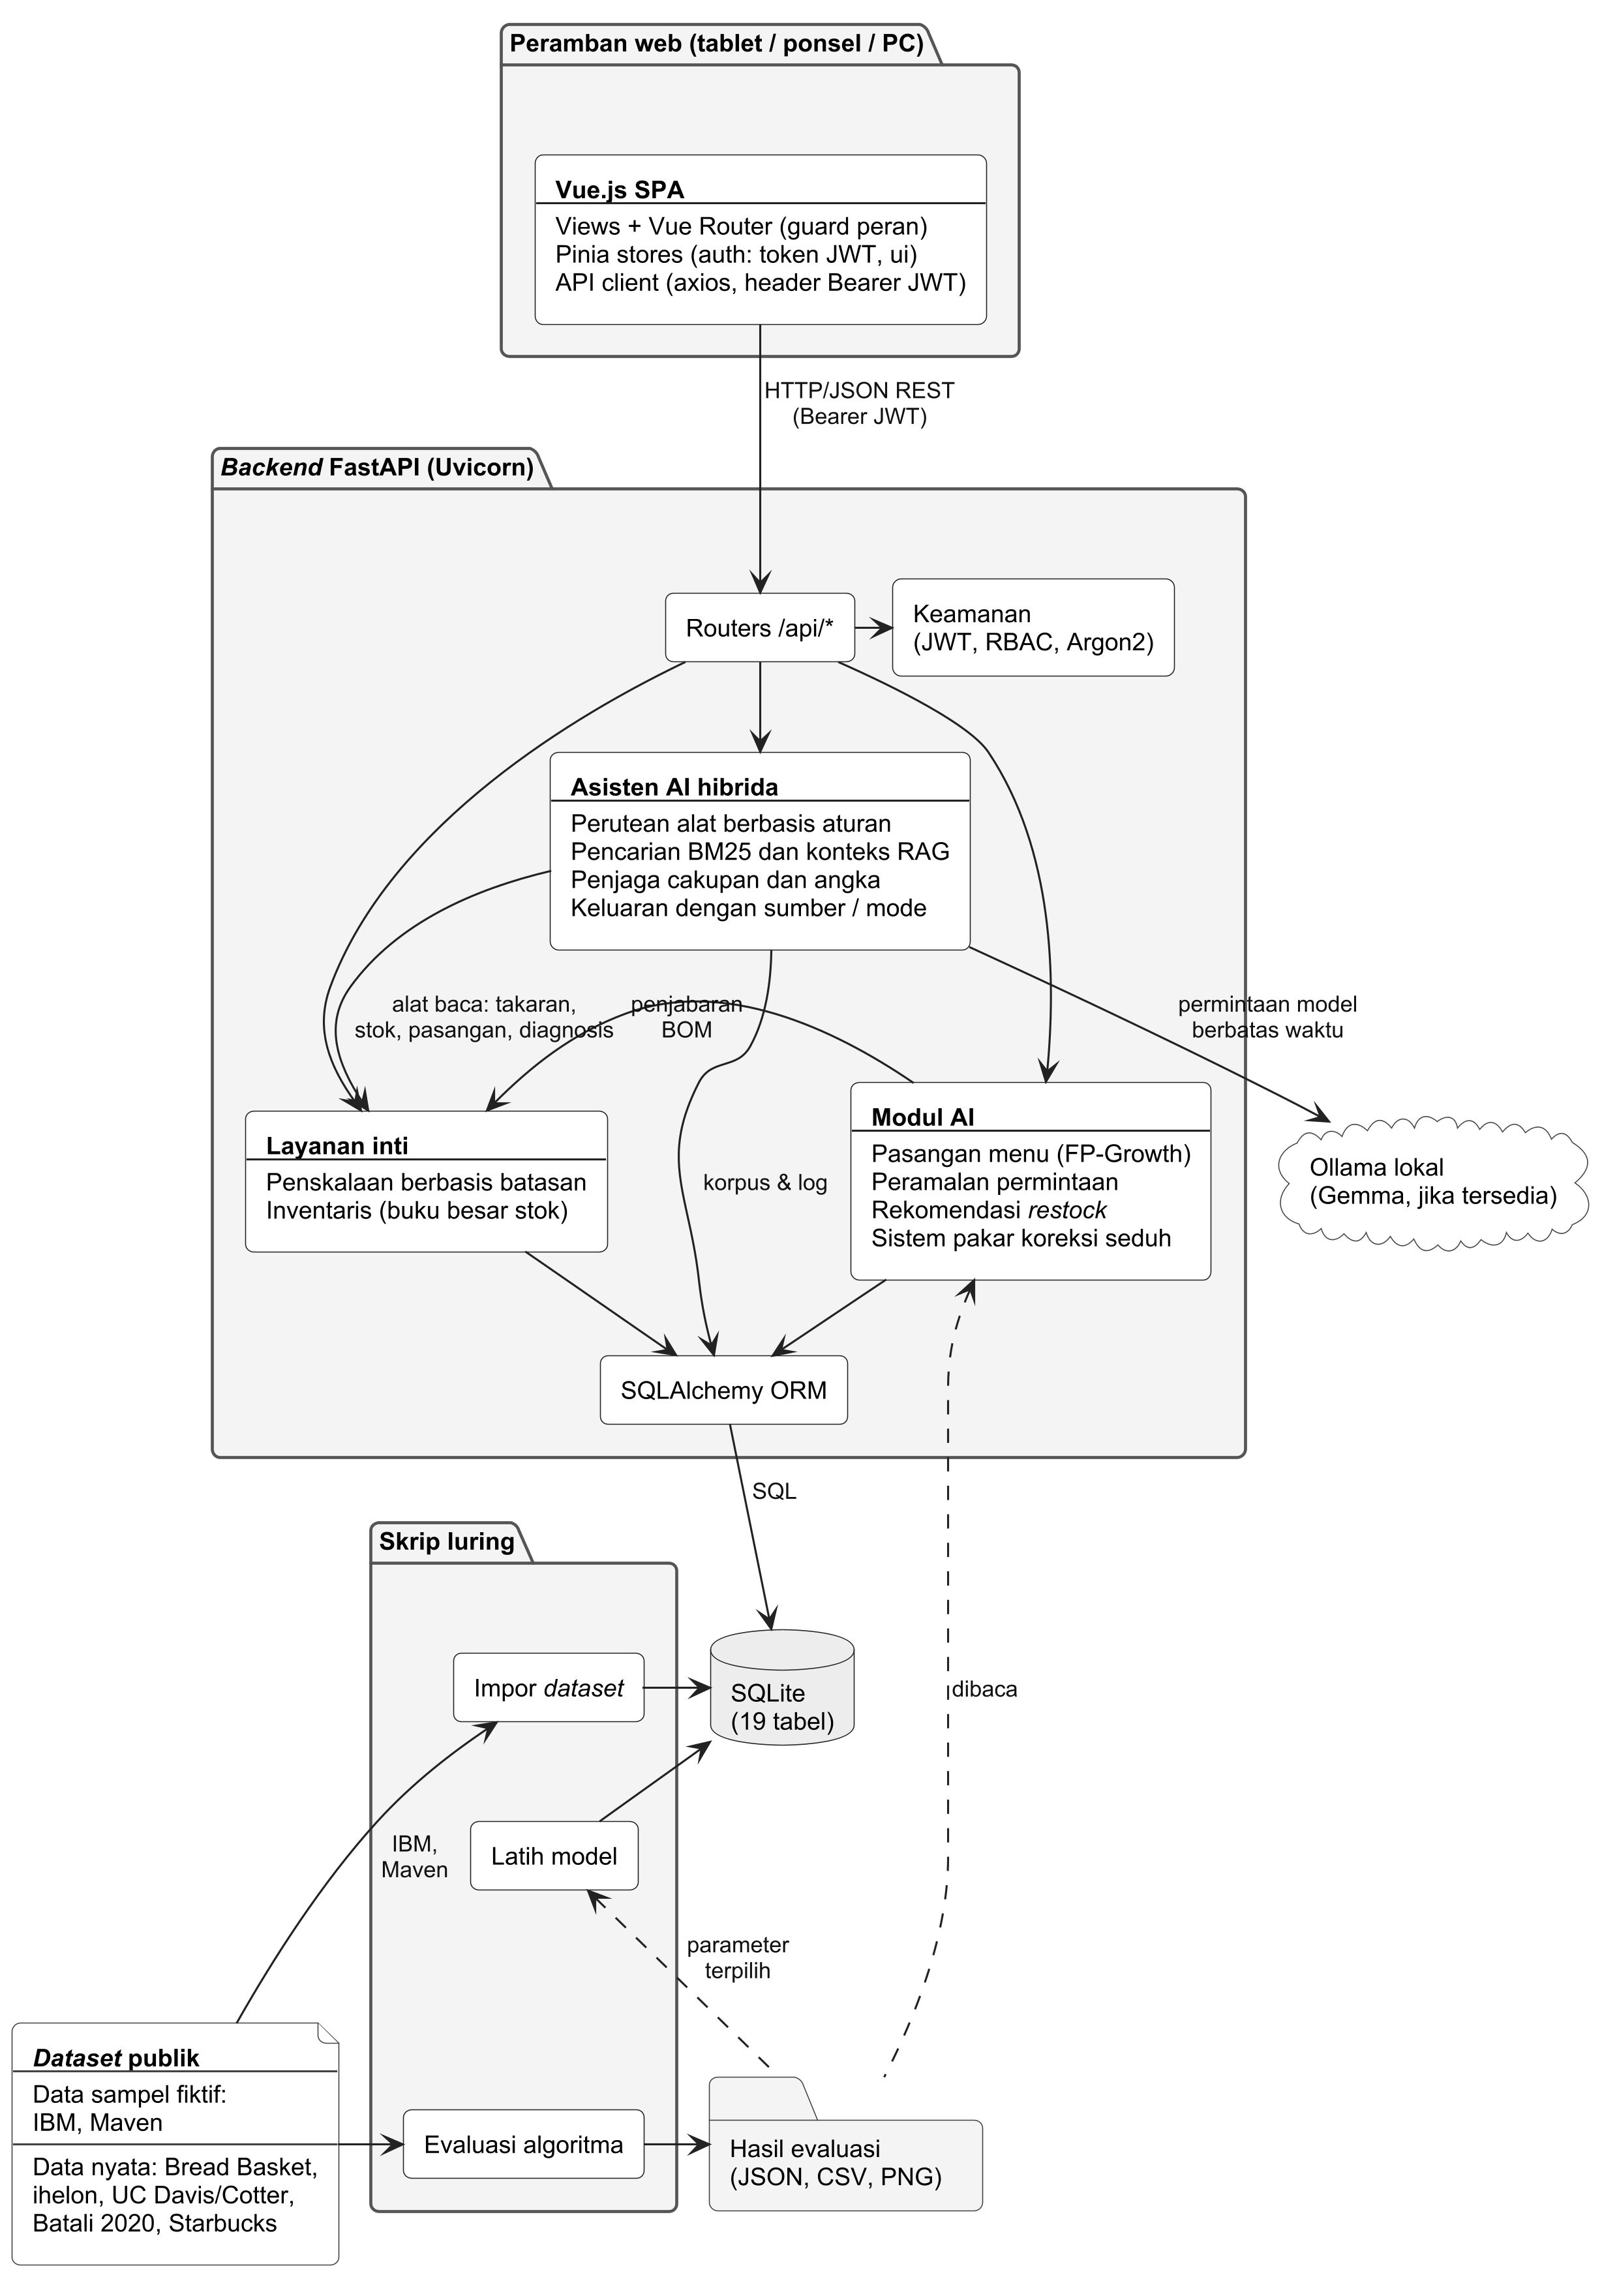
\includegraphics[width=.92\textwidth]{pic/arsitektur.png}
\caption{Arsitektur Aplikasi Takar}
\label{fig:arsitektur}
\end{figure}

Hubungan aktor dengan fungsi utama ditunjukkan pada Gambar~\ref{fig:use-case}. Alur kalkulator pada Gambar~\ref{fig:activity-kalkulator} berakhir pada pratinjau kebutuhan bahan dan peringatan; pengguna masih harus memilih tindakan catat produksi. Sesudah dicatat, setiap komponen resep turunan diuraikan menjadi bahan dasar dan ditulis sebagai pergerakan stok. Diagram sekuens pada Gambar~\ref{fig:sequence-produce} memperlihatkan bahwa perhitungan, log produksi, dan mutasi stok berada di sisi server sehingga tampilan yang ditutup tidak mengubah konsistensi catatan.

\begin{figure}[htbp]
\centering
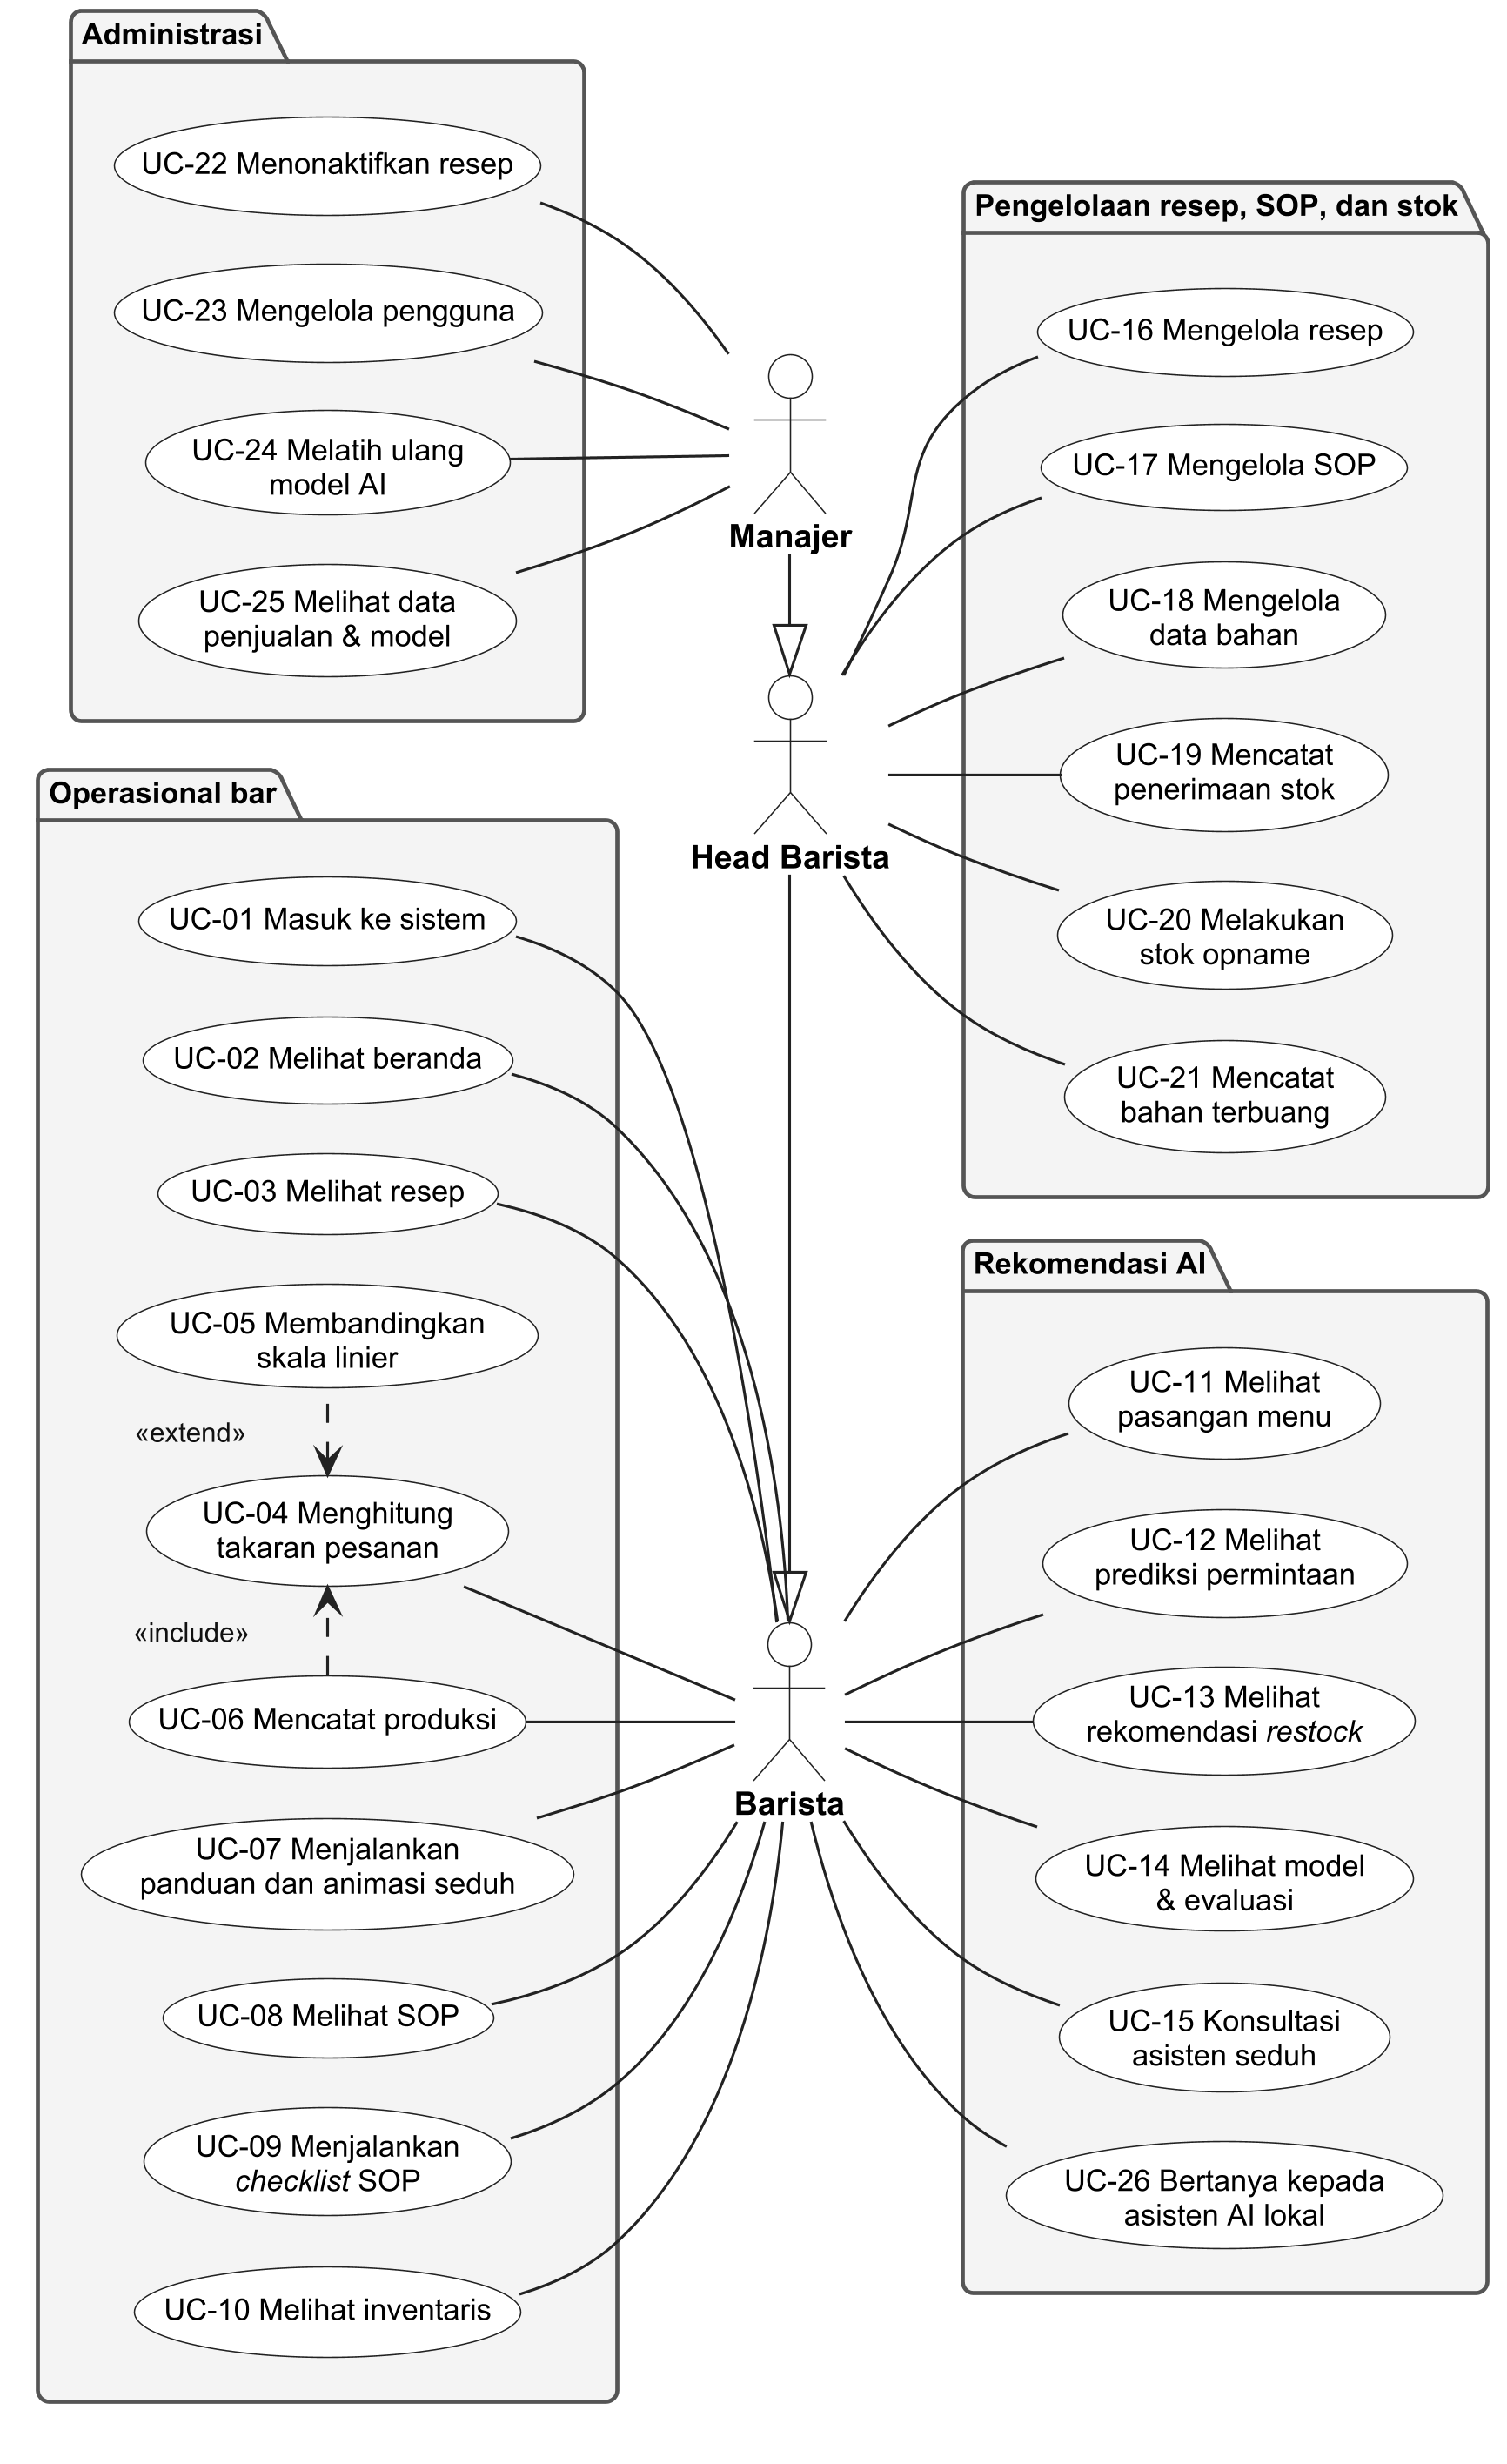
\includegraphics[width=.85\textwidth]{pic/use_case.png}
\caption{Kasus Penggunaan Menurut Peran}
\label{fig:use-case}
\end{figure}
\begin{figure}[htbp]
\centering
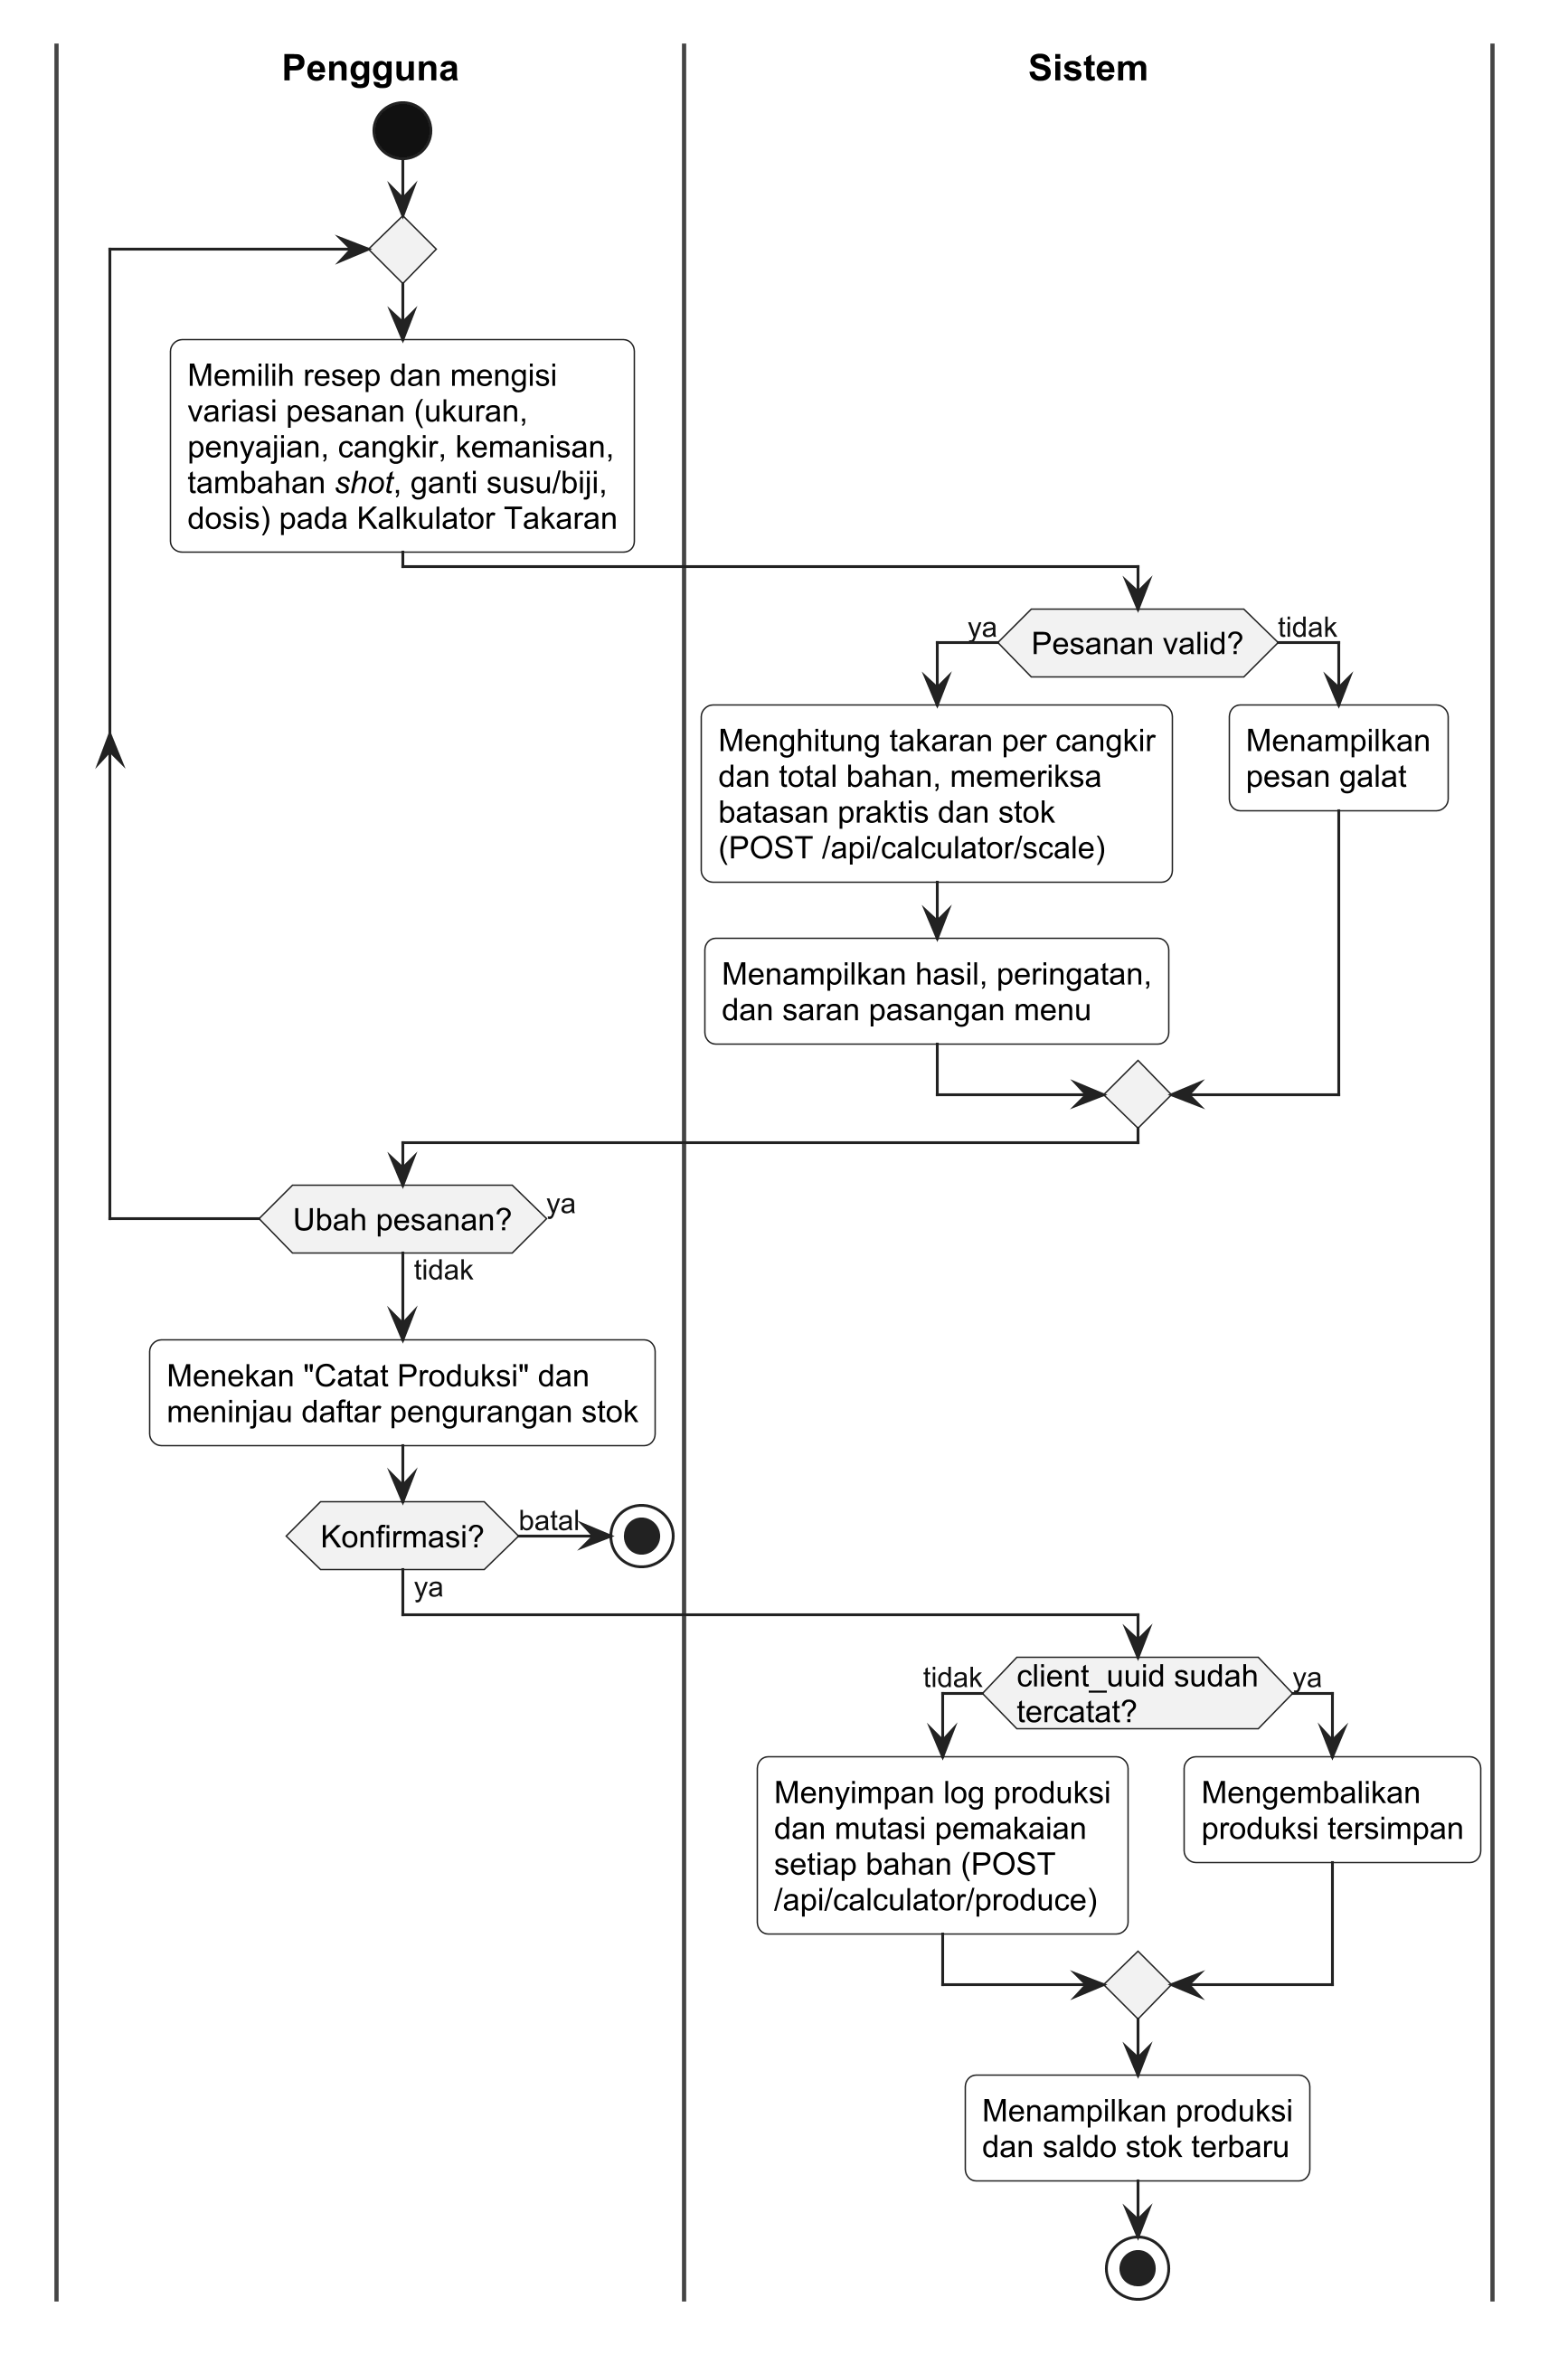
\includegraphics[width=.75\textwidth]{pic/activity_kalkulator.png}
\caption{Aktivitas Perhitungan Variasi Pesanan}
\label{fig:activity-kalkulator}
\end{figure}
\begin{figure}[htbp]
\centering
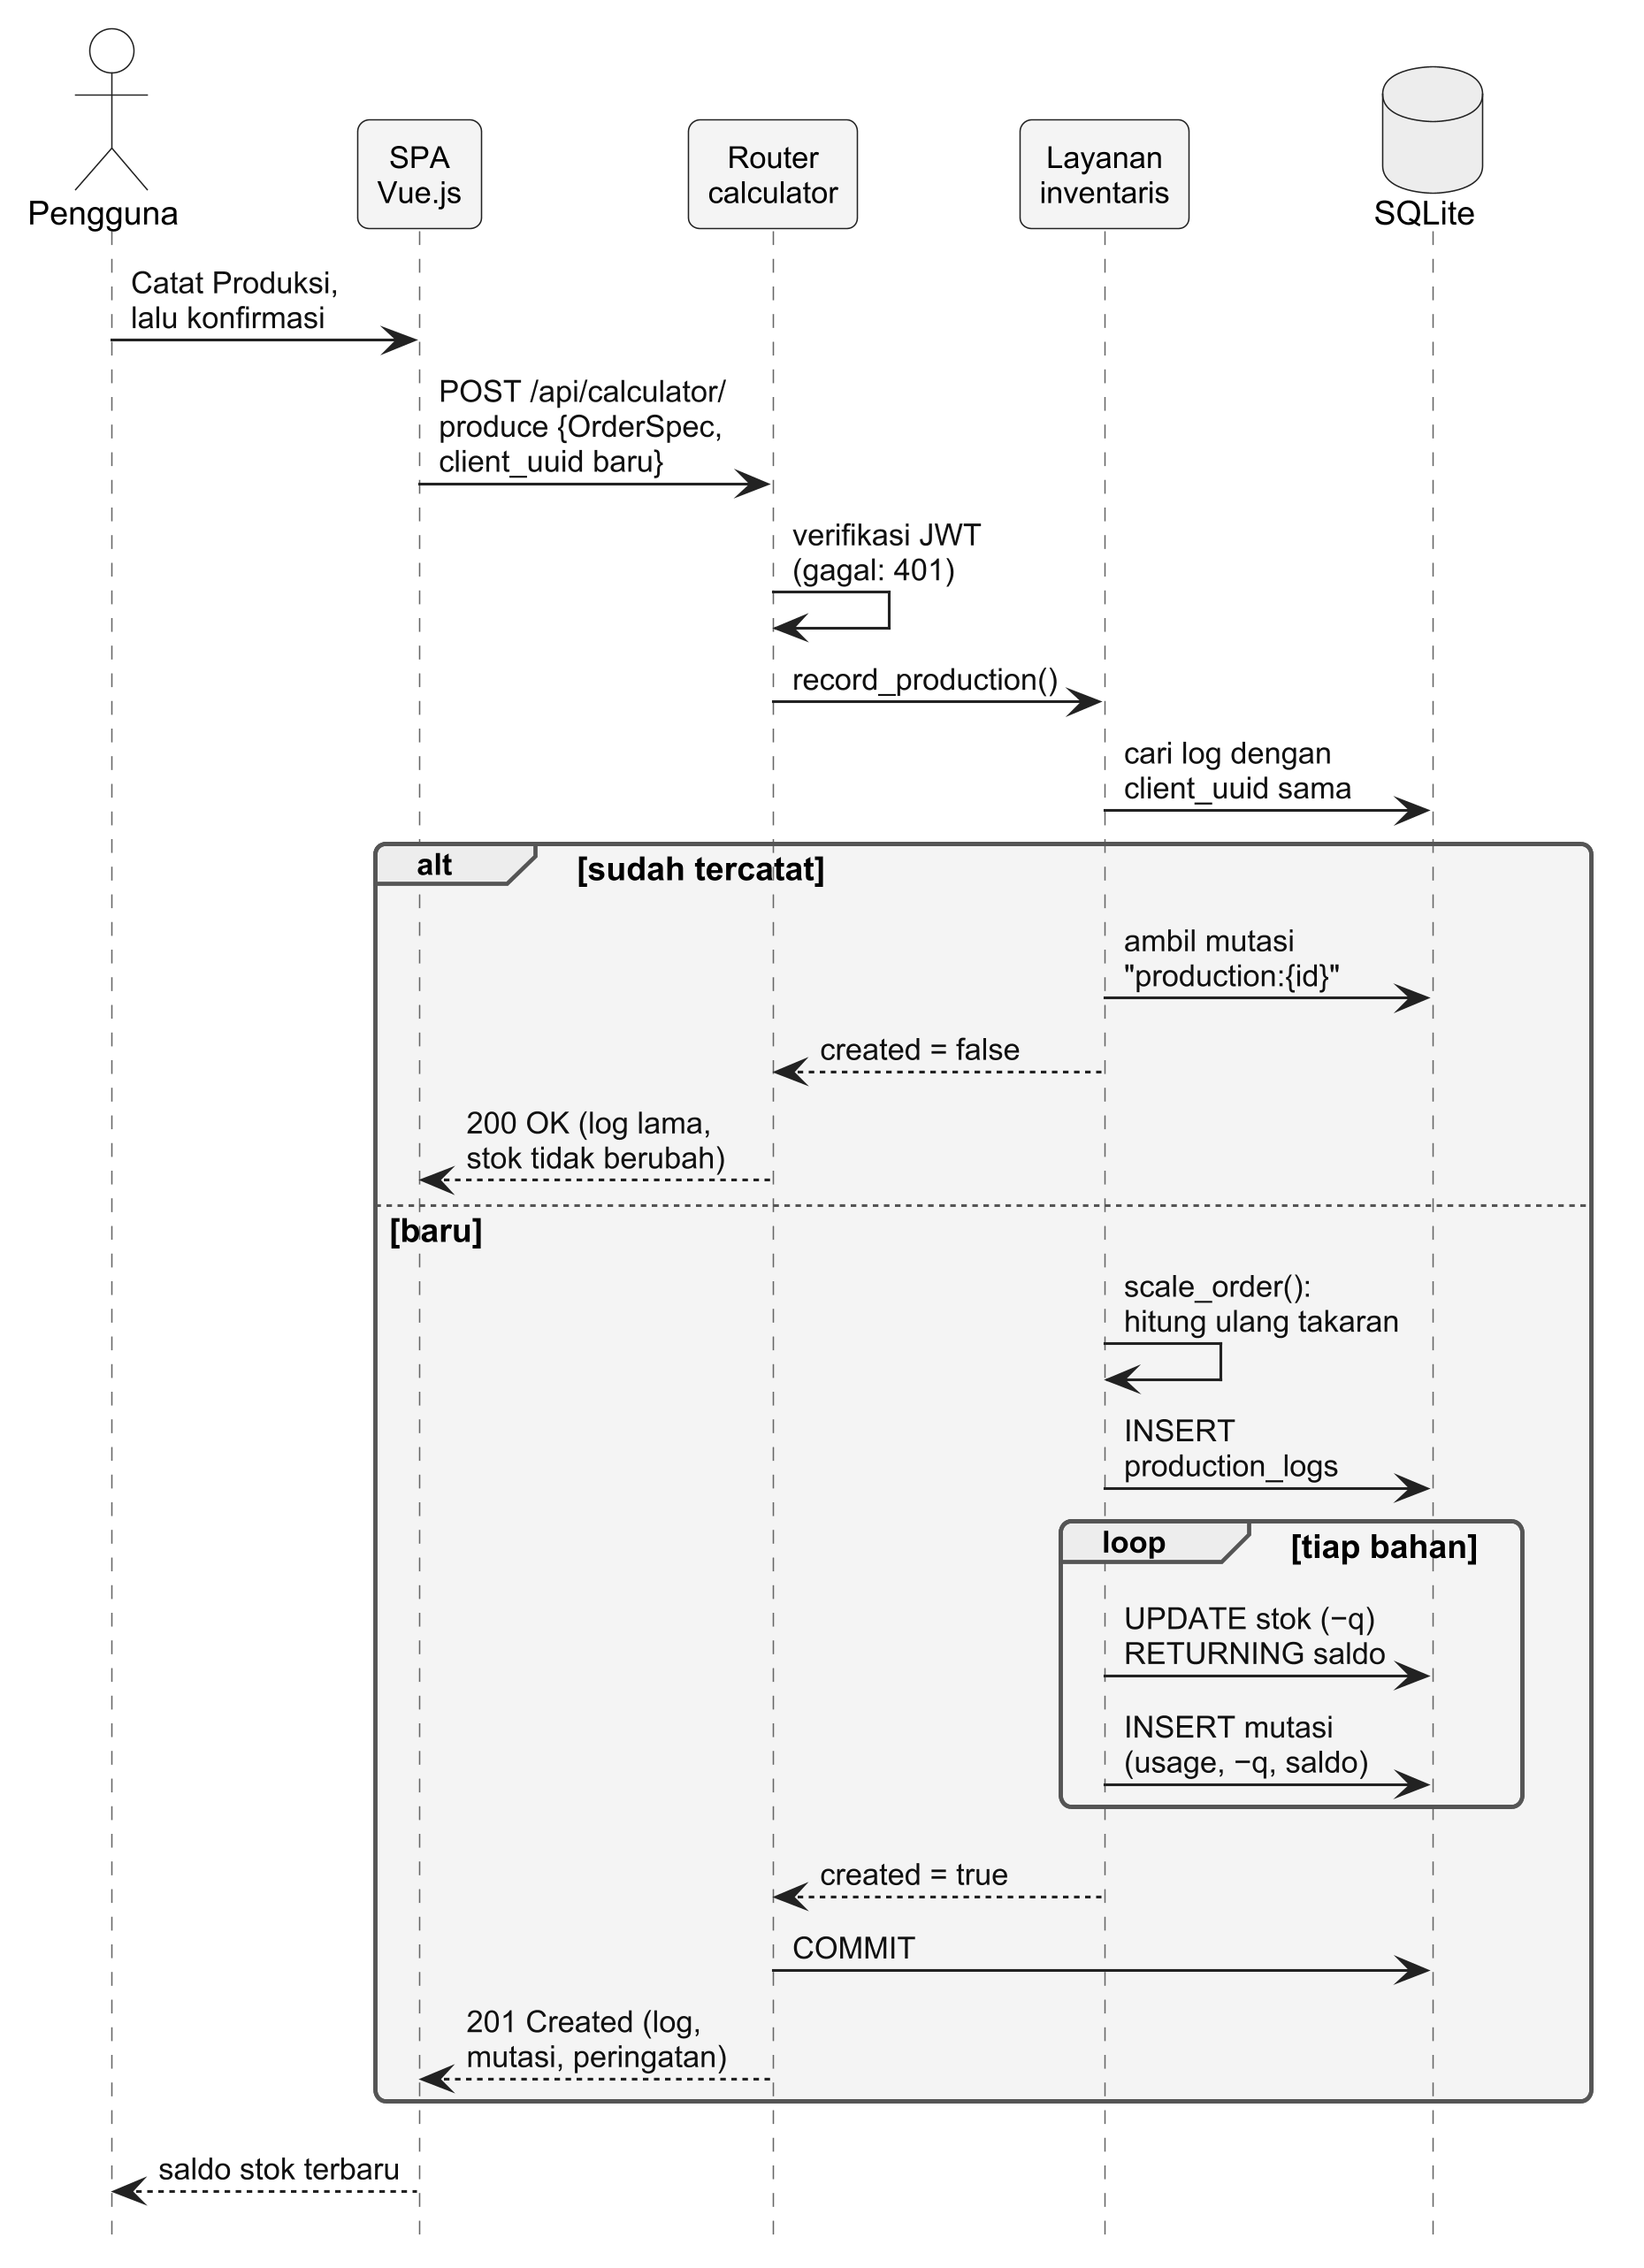
\includegraphics[width=.84\textwidth]{pic/sequence_produce.png}
\caption{Sekuens Pencatatan Produksi dan Pergerakan Stok}
\label{fig:sequence-produce}
\end{figure}

Rancangan data pada Gambar~\ref{fig:erd} menggunakan resep dan komponen sebagai daftar bahan (\textit{bill of materials}, BOM). Komponen dapat menunjuk bahan langsung atau subresep, misalnya satu \textit{shot} espreso yang memiliki kebutuhan biji sendiri. Ukuran resep menyimpan volume cangkir dan pengecualian jumlah \textit{shot} per ukuran. Tabel pergerakan inventaris menyimpan kuantitas bertanda dan saldo setelah transaksi; stok bahan berubah hanya lewat layanan pencatatan pergerakan. Tabel penjualan, aturan pasangan, prakiraan, dan riwayat pelatihan mendukung model AI tanpa menggabungkan transaksi dataset publik dengan produksi kedai demo. Log asisten menyimpan pertanyaan, jawaban, mode, rujukan, alat yang digunakan, dan latensi untuk penelusuran kesalahan pada instalasi lokal.

\begin{figure}[htbp]
\centering
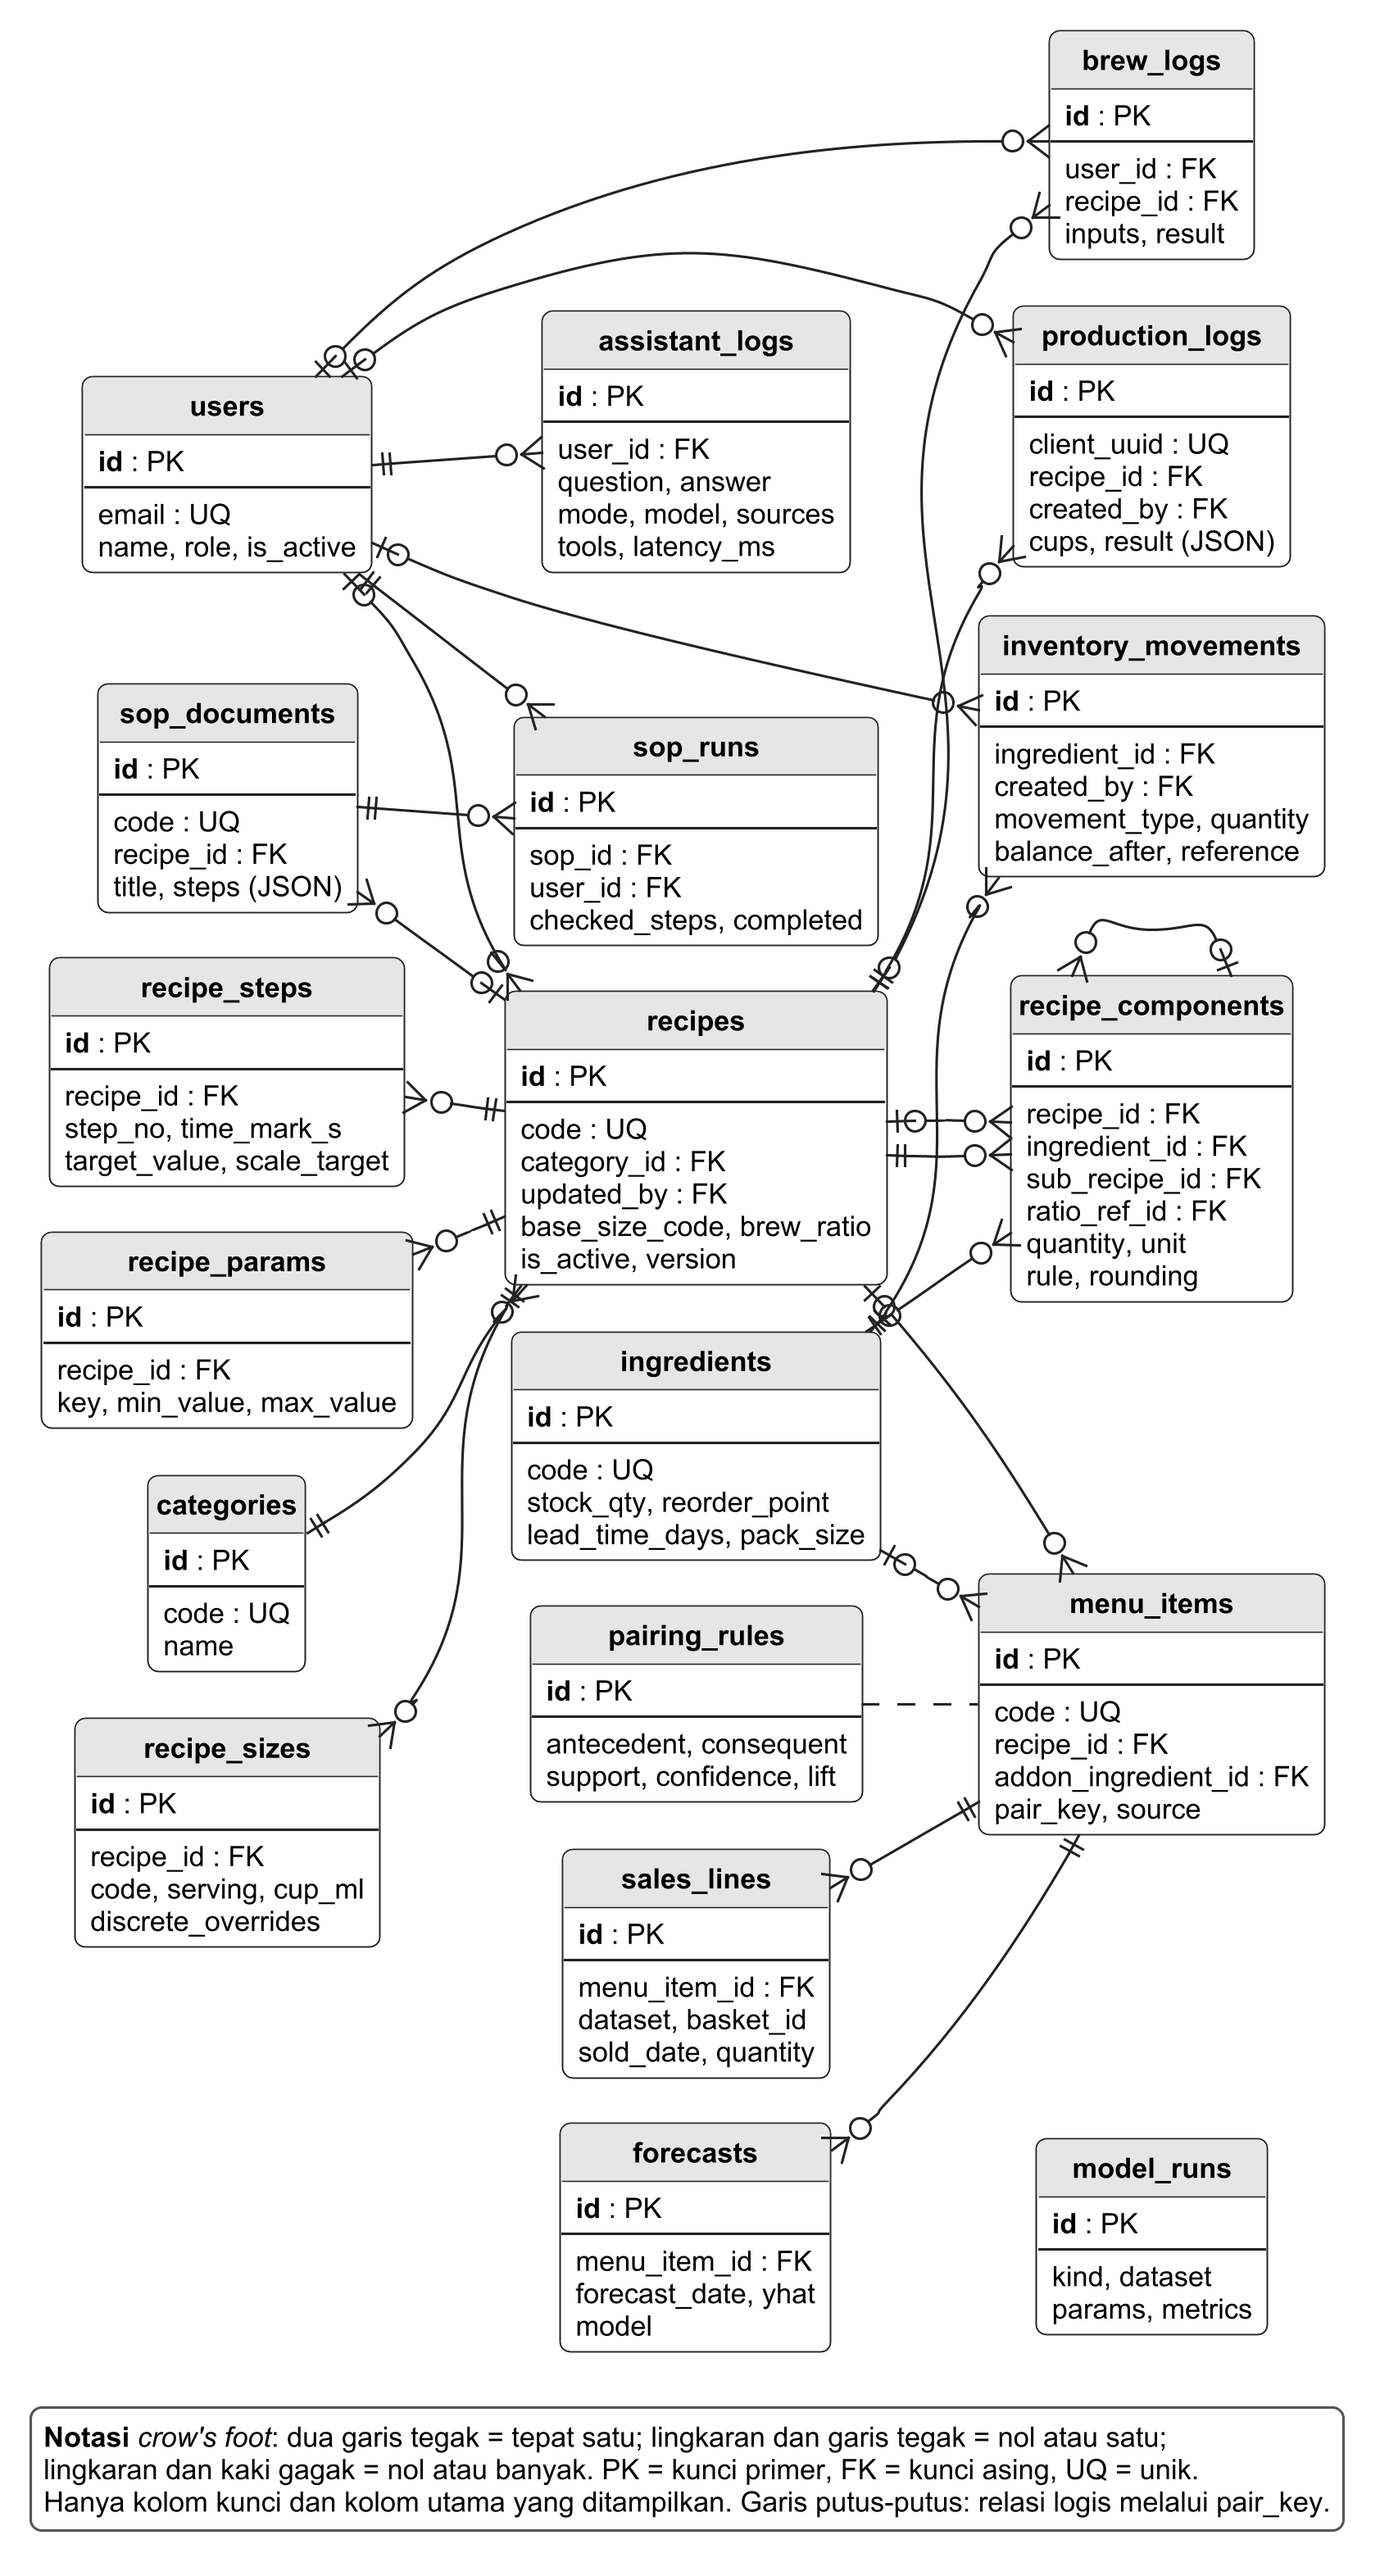
\includegraphics[width=.86\textwidth]{pic/erd.png}
\caption{Rancangan Entitas dan Relasi Basis Data Takar}
\label{fig:erd}
\end{figure}

Kontrak layanan utama dirangkum pada Tabel~\ref{tab:endpoint}. Seluruh alamat pada tabel memakai awalan \texttt{/api}. Permintaan tanpa token atau dengan peran yang tidak berhak dikembalikan sebagai HTTP 401 atau 403; masukan yang tidak memenuhi aturan dikembalikan sebagai HTTP 422. Pencatatan produksi memakai pengenal permintaan klien untuk mencegah pengurangan stok berulang akibat pengiriman ulang.

\begin{table}[htbp]
\centering
\caption{Kelompok \textit{Endpoint} API Utama}
\label{tab:endpoint}
\begin{tabular}{p{.27\textwidth}p{.59\textwidth}}
\toprule
Kelompok & Fungsi \\
\midrule
\texttt{/auth}, \texttt{/users} & Masuk, identitas sesi, dan pengelolaan pengguna. \\
\texttt{/recipes}, \texttt{/sop} & Katalog, detail, perubahan resep dan SOP, serta checklist. \\
\texttt{/calculator} & Penskalaan, pembanding linier, produksi, dan riwayat. \\
\texttt{/ingredients}, \texttt{/inventory} & Data bahan, stok, penerimaan, penyesuaian, limbah, dan buku besar. \\
\texttt{/ai}, \texttt{/sales} & Pasangan menu, peramalan, \textit{restock}, diagnosis seduh, model, dan ringkasan transaksi. \\
\texttt{/dashboard}, \texttt{/assistant} & Ringkasan operasional dan layanan asisten tanya-jawab lokal. \\
\bottomrule
\end{tabular}
\end{table}

Peta navigasi pada Gambar~\ref{fig:peta-situs} menempatkan kalkulator dan panduan seduh dekat detail resep agar barista dapat beralih dari membaca standar ke menjalankannya. Menu manajemen resep, inventaris, data model, dan pengguna mengikuti hak akses. Komponen tampilan menyajikan status kosong dan kesalahan secara jelas, termasuk saat model belum dilatih atau layanan model bahasa lokal tidak tersedia.

\begin{figure}[htbp]
\centering
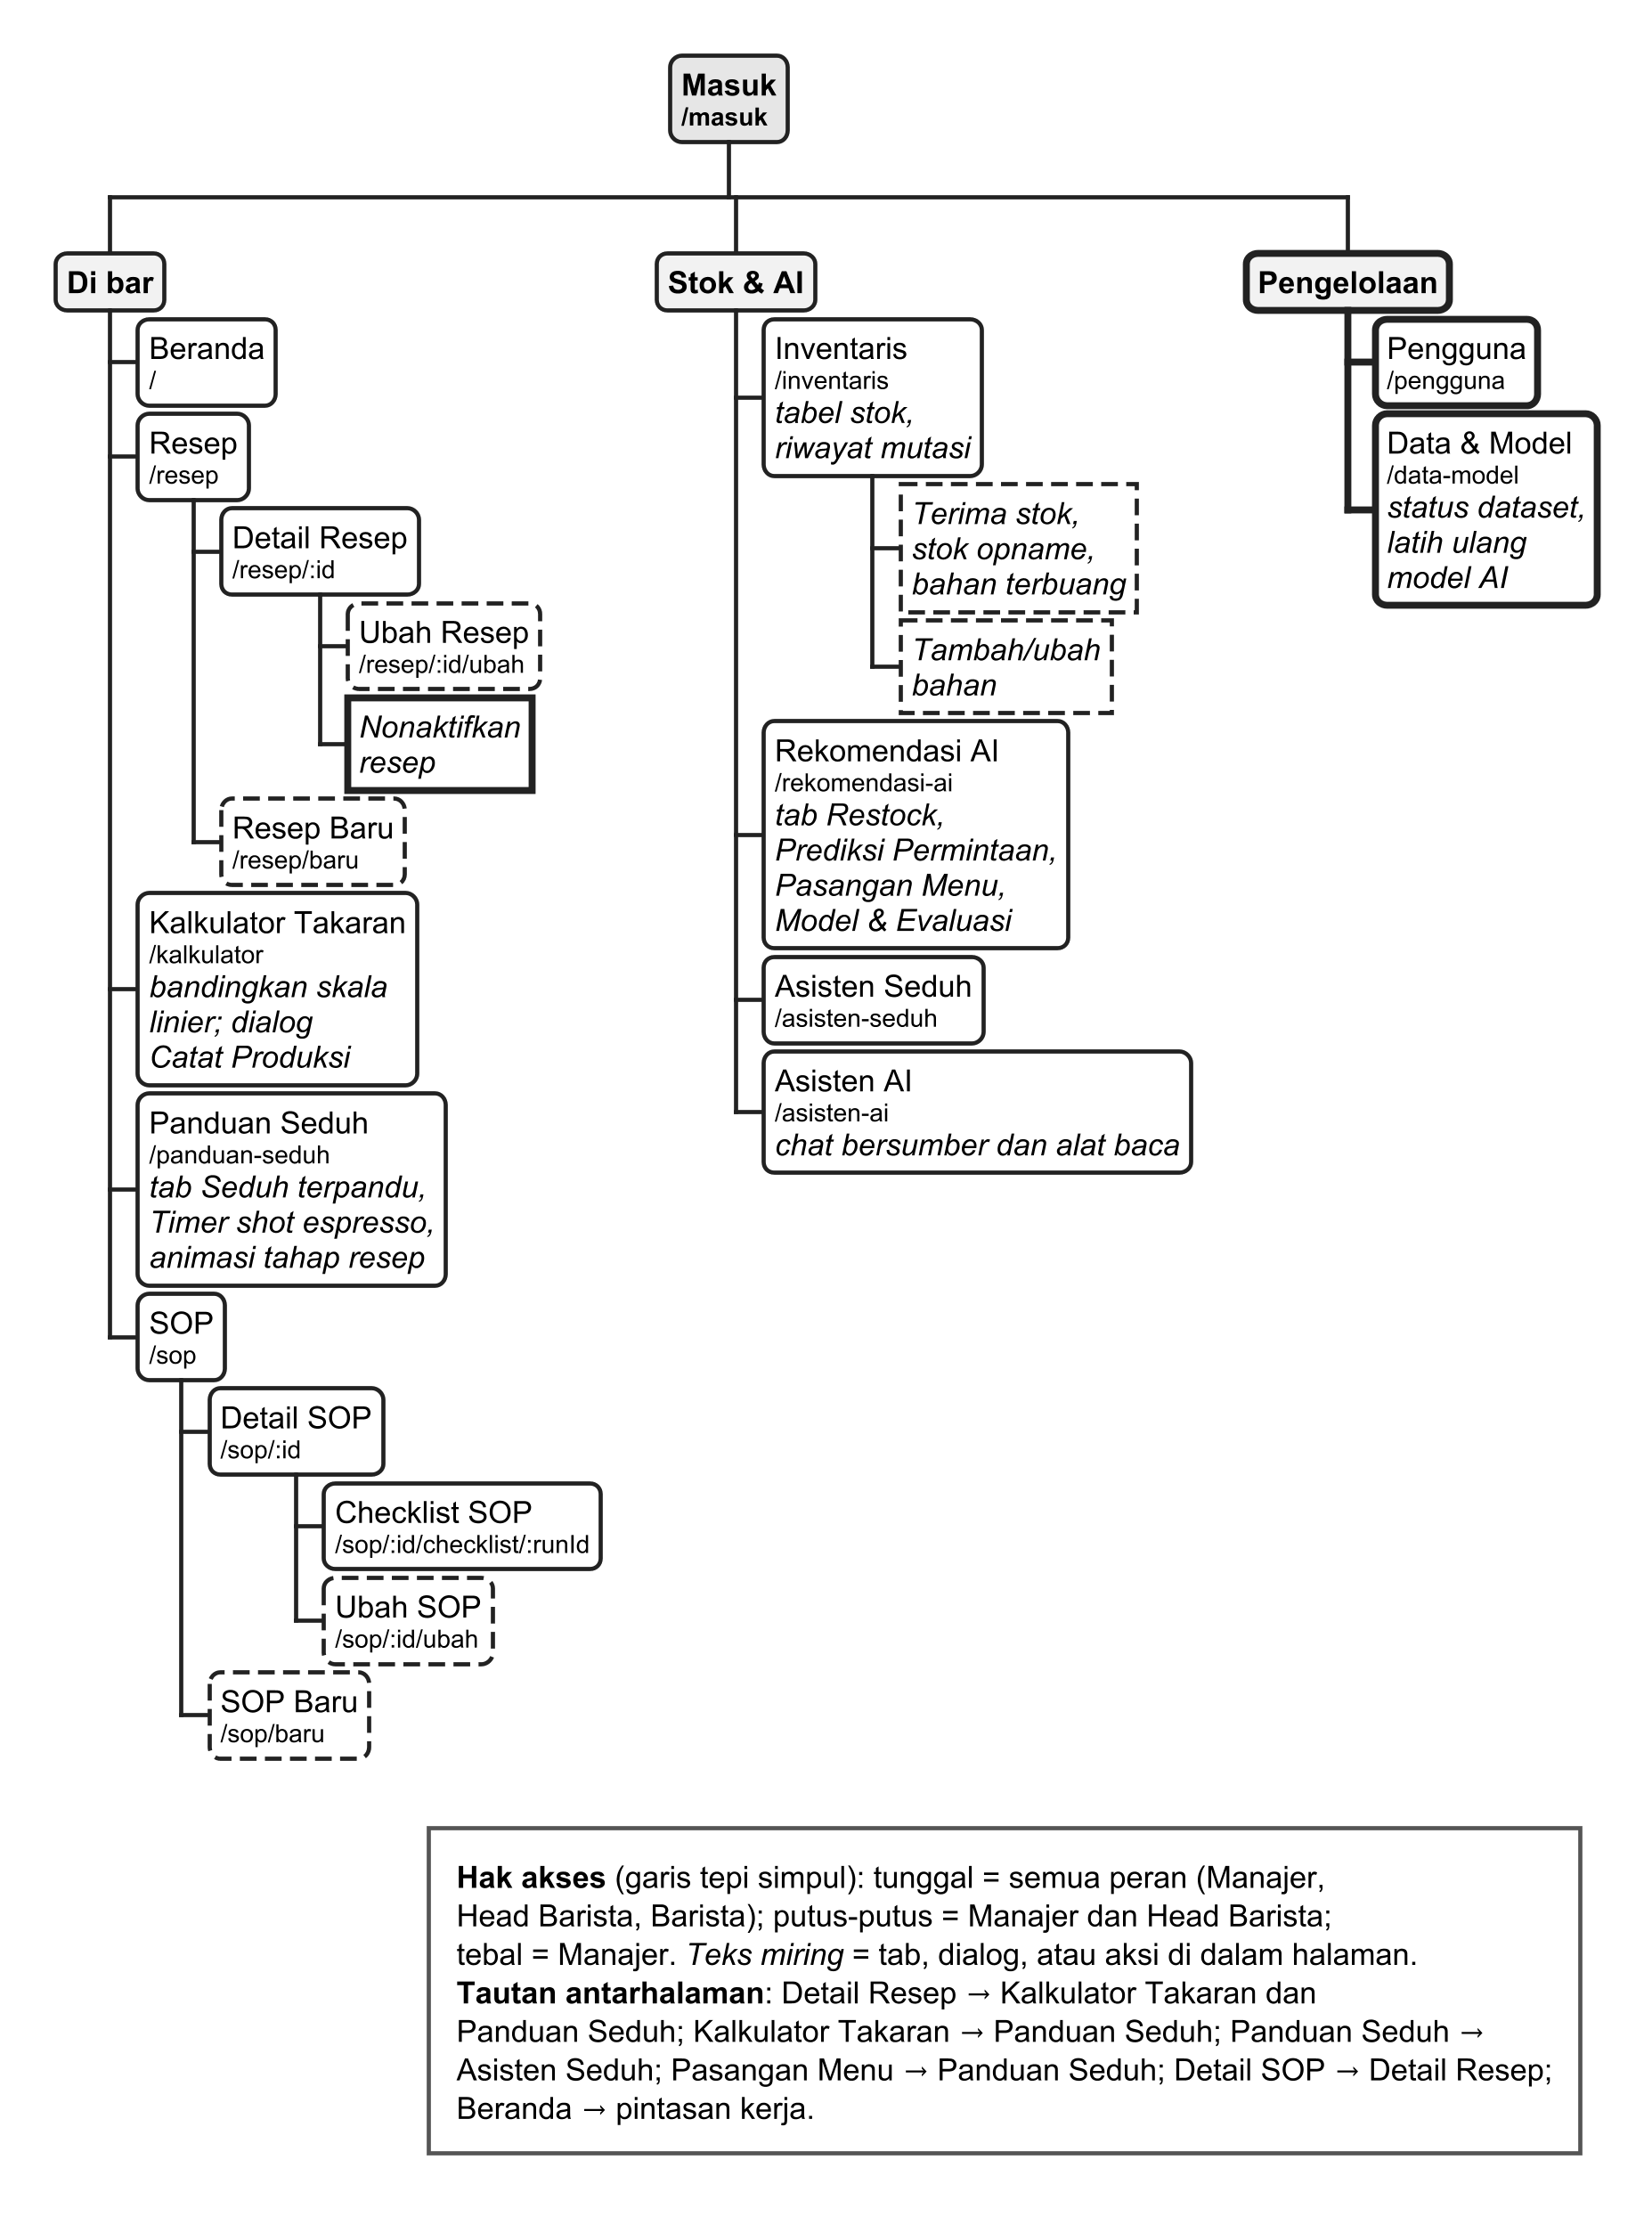
\includegraphics[width=.85\textwidth]{pic/peta_situs.png}
\caption{Peta Navigasi Aplikasi}
\label{fig:peta-situs}
\end{figure}

\section{Perancangan Algoritma}
\label{sec:perancangan-algoritma}

\subsection{Penskalaan Resep Berbasis Batasan}

Setiap resep memiliki ukuran dasar dan aturan untuk setiap komponen. Untuk ukuran yang dipilih, faktor awal adalah volume cangkir yang diminta dibagi volume dasar. Pada V60, dosis yang diminta mengganti faktor tersebut dengan rasio dosis baru terhadap dosis dasar. Komponen proporsional dikalikan faktor; komponen tetap tidak berubah; \textit{shot} dibulatkan ke kelipatan utuh atau mengikuti tabel pengecualian ukuran. Pemanis mengikuti persentase manis. Air dengan aturan rasio dihitung sesudah dosis akhir diketahui, sedangkan susu pengisi dihitung setelah volume komponen lain agar tidak melampaui cangkir.

Algoritma~\ref{alg:penskalaan} menyatakan urutan ketergantungan tersebut. Pembulatan mengikuti ketelitian takar masing-masing bahan. Target tuang kumulatif V60 ikut diskalakan, sedangkan waktu penanda langkah tetap. Jika es dan bahan lain sudah memenuhi cangkir, jumlah es dapat dikurangi; pesanan dengan komponen pengisi yang tetap melampaui batas ditolak. Subresep kemudian diuraikan menjadi bahan dasar per cangkir dan dikalikan jumlah cangkir, sehingga jumlah total tepat merupakan kelipatan takaran per cangkir. Pemeriksaan menghasilkan peringatan untuk luapan, kurang isi, perubahan rasio, dosis di luar rentang, dan stok yang kurang.

\begin{algorithm}[htbp]
\caption{Penskalaan Resep Berbasis Batasan}
\label{alg:penskalaan}
\begin{algorithmic}[1]
\Require resep, ukuran, sajian, jumlah cangkir, manis, \textit{shot}, pertukaran bahan, dosis
\Ensure takaran per cangkir, kebutuhan total, langkah, dan peringatan
\State Tentukan volume cangkir dan faktor ukuran atau faktor dosis
\State Pilih komponen sajian; terapkan pertukaran yang sah
\For{setiap komponen proporsional, tetap, dan diskret}
  \State Hitung menurut aturan; terapkan manis dan tambahan \textit{shot}
  \State Bulatkan ke ketelitian takar komponen
\EndFor
\For{setiap komponen rasio}
  \State Hitung dari komponen acuan yang sudah final
\EndFor
\State Hitung ruang setelah volume bahan lain dan es diperiksa
\State Isi komponen \textit{top up}; tolak pesanan yang tidak muat
\State Skala target langkah dan periksa seluruh batasan
\State Uraikan subresep menjadi bahan dasar per cangkir
\State Kalikan kebutuhan per cangkir dengan jumlah cangkir
\State \Return hasil dan peringatan
\end{algorithmic}
\end{algorithm}

Gambar~\ref{fig:alur-penskalaan} merinci cabang aturan untuk komponen yang berbeda. Pembanding pertama adalah penskalaan linier mentah yang mengalikan semua kuantitas dasar dengan faktor. Pembanding kedua membulatkan hasil linier ke ketelitian takar, termasuk \textit{shot}, tetapi tidak memperhitungkan pengisian dan ruang cangkir. Pembanding kedua memisahkan efek pembulatan dari efek aturan kapasitas. Ketiganya dinilai pada pesanan yang setara.

\begin{figure}[htbp]
\centering
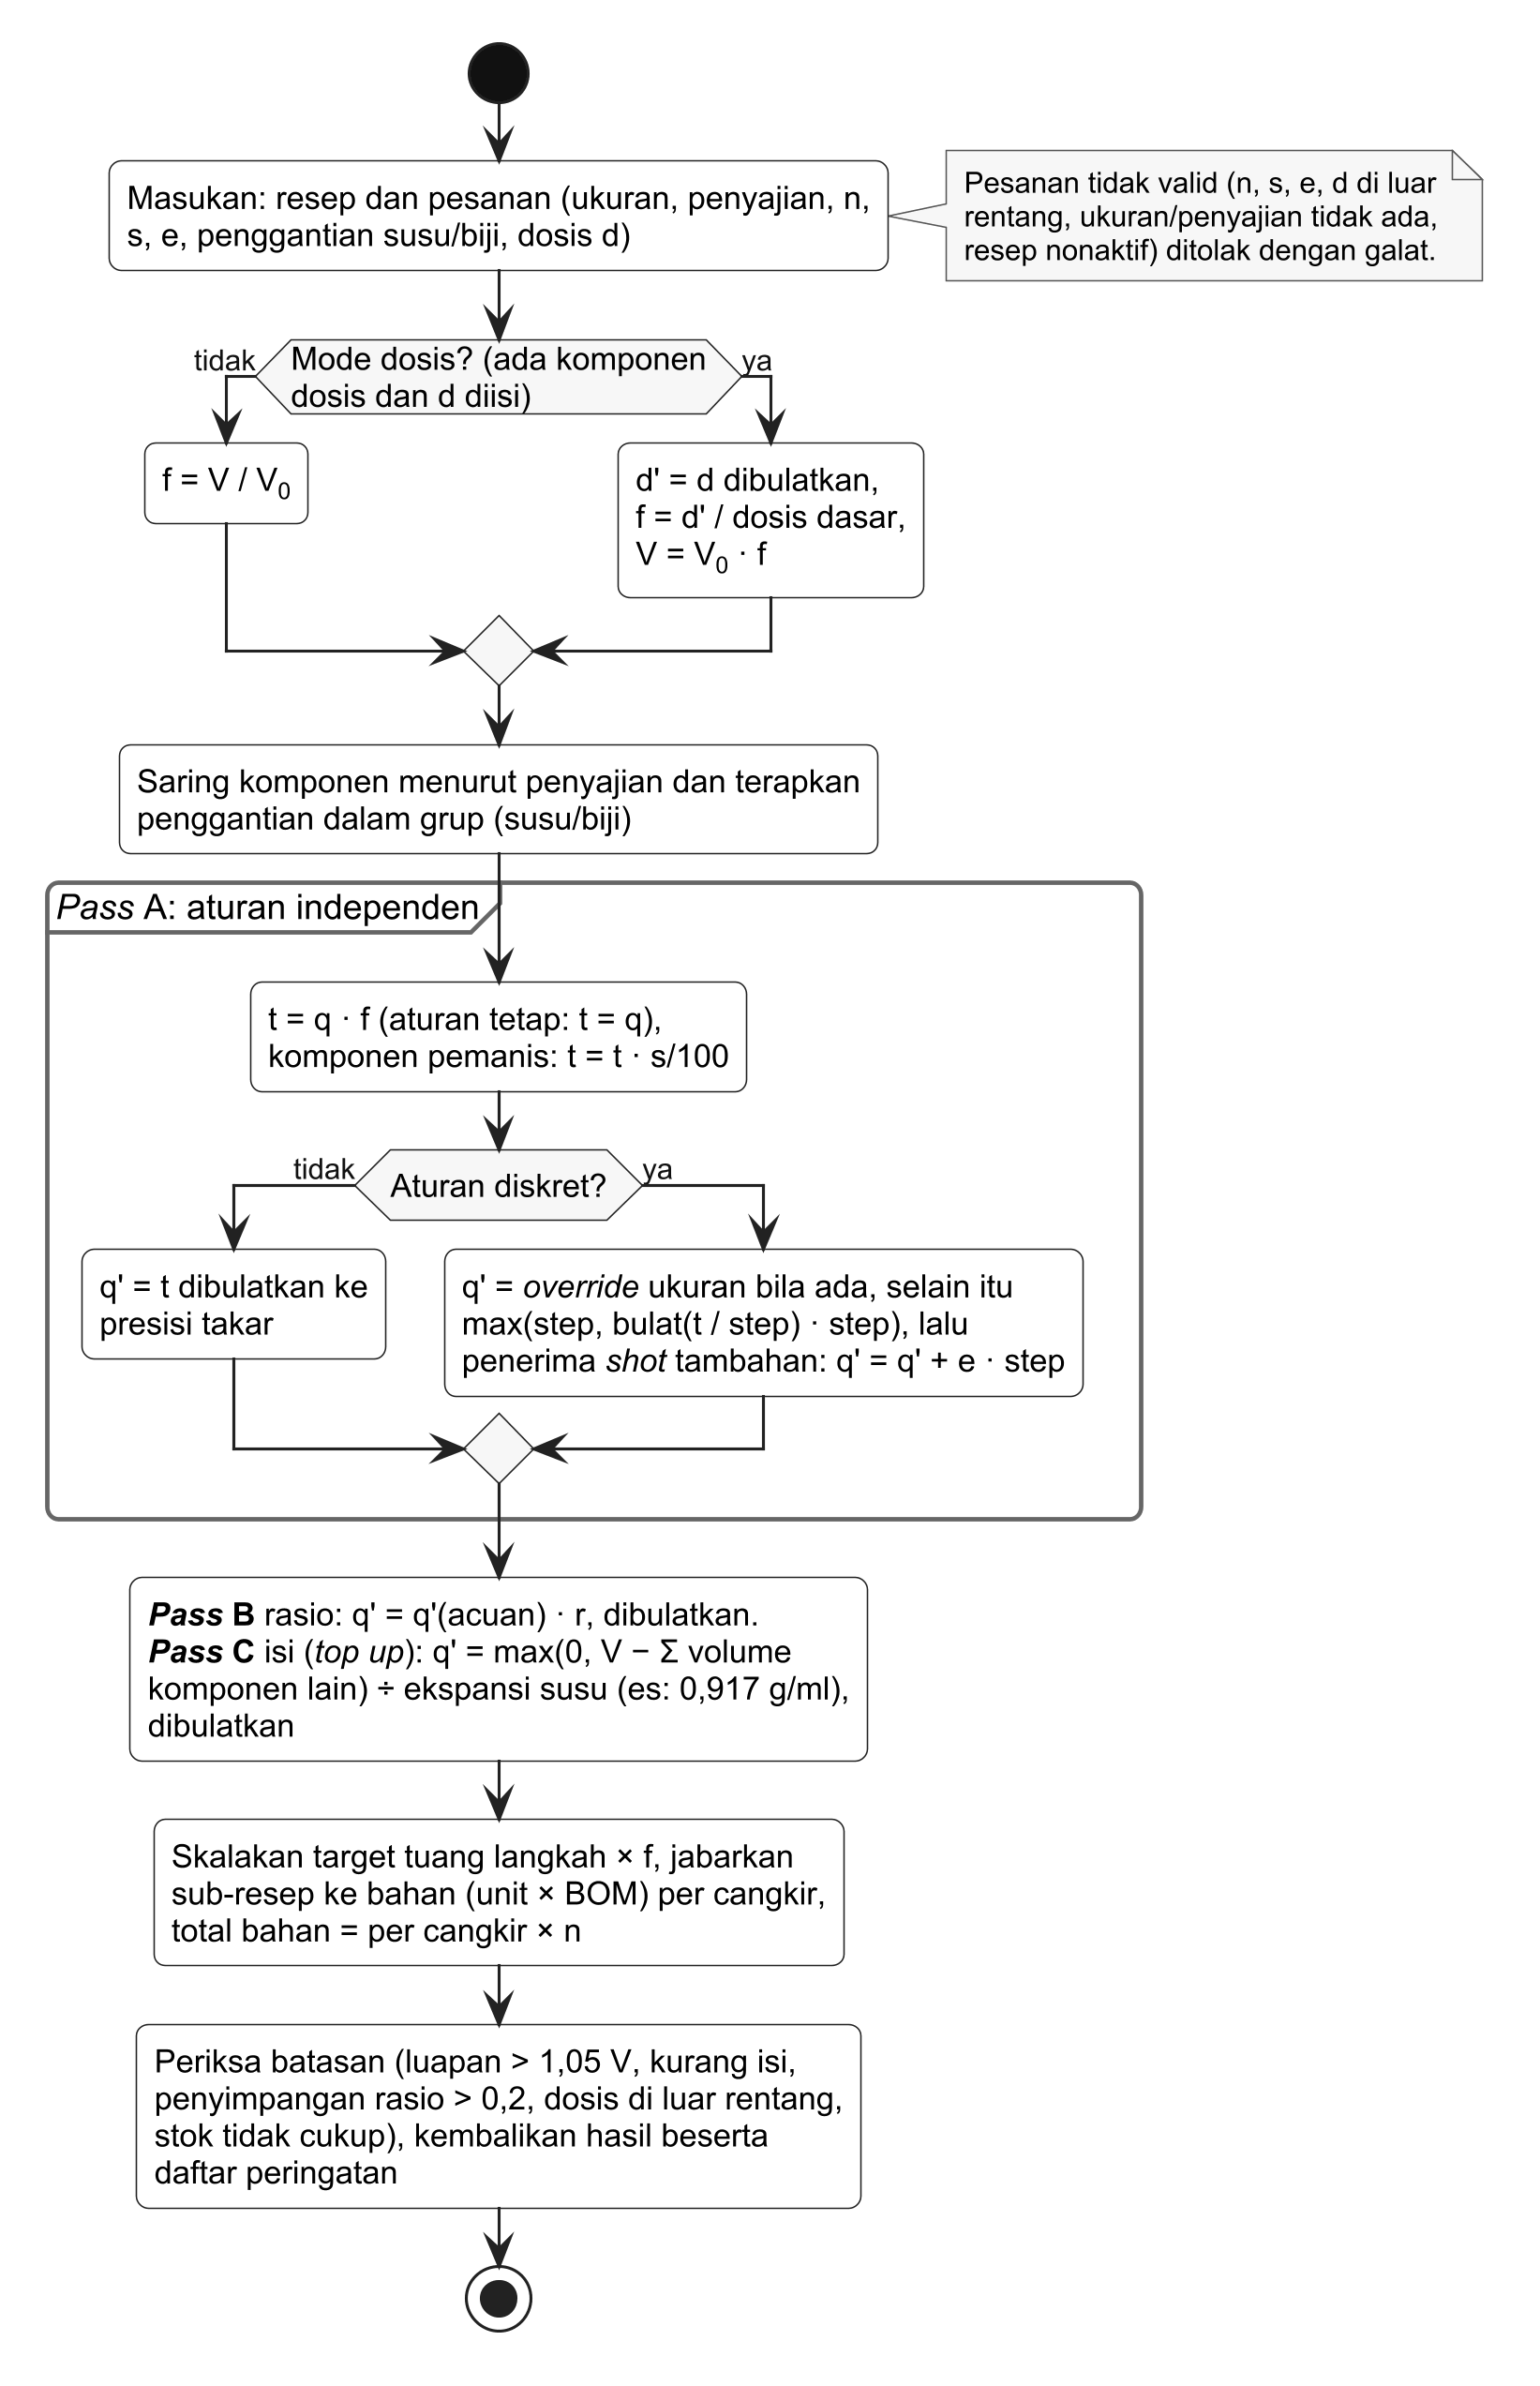
\includegraphics[width=.88\textwidth]{pic/alur_penskalaan.png}
\caption{Alur Aturan Penskalaan dan Pemeriksaan Batasan}
\label{fig:alur-penskalaan}
\end{figure}

\subsection{Pasangan Menu dan Peramalan}

Transaksi IBM dibentuk menjadi keranjang berdasarkan outlet, tanggal, dan nomor struk. Produk dengan ukuran berbeda dinormalisasi menjadi kunci menu yang sama, lalu FP-Growth menambang itemset dan aturan asosiasi. Rekomendasi menerima item yang sedang dipilih, mencocokkan anteseden aturan, mengurutkan konsekuen menurut \textit{confidence} kemudian \textit{lift}, menghapus duplikat, dan mengisi kekurangan tempat dengan item populer yang ditandai sebagai isian. Aplikasi hanya menampilkan aturan dengan \textit{lift} lebih besar dari satu; seluruh aturan tanpa saringan dinilai tersendiri sebagai ablasi. Produk resep yang tidak ada dalam dataset dapat memakai kunci proksi yang dinyatakan di antarmuka.

Peramalan mengubah baris penjualan Maven menjadi deret unit harian per produk dan outlet, dengan tanggal tanpa transaksi diberi nilai nol. Enam metode dibandingkan: \textit{naive}, \textit{seasonal naive} mingguan, rata-rata bergerak tujuh hari, \textit{simple exponential smoothing}, Holt-Winters aditif, dan \textit{histogram gradient boosting} global. Fitur model global hanya memakai lag dan ringkasan penjualan yang telah tersedia di titik asal ramalan. Setiap origin dilatih ulang dengan data sampai origin tersebut, kemudian menghasilkan tujuh hari ke depan. Model aplikasi dipilih menurut WAPE keseluruhan terendah pada data pengembangan.

\subsection{Rekomendasi Pengisian Ulang}

Prakiraan produk diterjemahkan ke kebutuhan bahan melalui BOM resep. Bagi bahan $i$, kebutuhan selama \textit{lead time} $L_i$ adalah penjumlahan kebutuhan harian yang diramalkan, sedangkan simpangan baku galat harian dari periode kalibrasi digunakan untuk stok pengaman. Dengan periode tinjau $R=1$ hari dan koefisien layanan contoh $z=1{,}65$, rancangan memakai
\begin{equation}
SS_i=z\sigma_i\sqrt{L_i},\qquad
ROP_i=\widehat D_i(L_i)+SS_i,\qquad
S_i=\widehat D_i(L_i+R)+SS_i.
\label{eq:restock}
\end{equation}
Di sini $\widehat D_i(h)$ adalah akumulasi kebutuhan ramalan selama $h$ hari, $\sigma_i$ simpangan baku galat harian, $ROP_i$ titik pemesanan ulang, dan $S_i$ tingkat persediaan sasaran. Jumlah yang disarankan adalah selisih positif antara $S_i$ dan posisi stok, dibulatkan ke ukuran kemasan. Angka $z$, \textit{lead time}, dan ukuran kemasan dalam demonstrasi merupakan asumsi, bukan hasil pengukuran pemasok kedai. Gambar~\ref{fig:sequence-restock} memperlihatkan aliran dari ramalan produk menuju kebutuhan bahan dan saran pesan.

\begin{figure}[htbp]
\centering
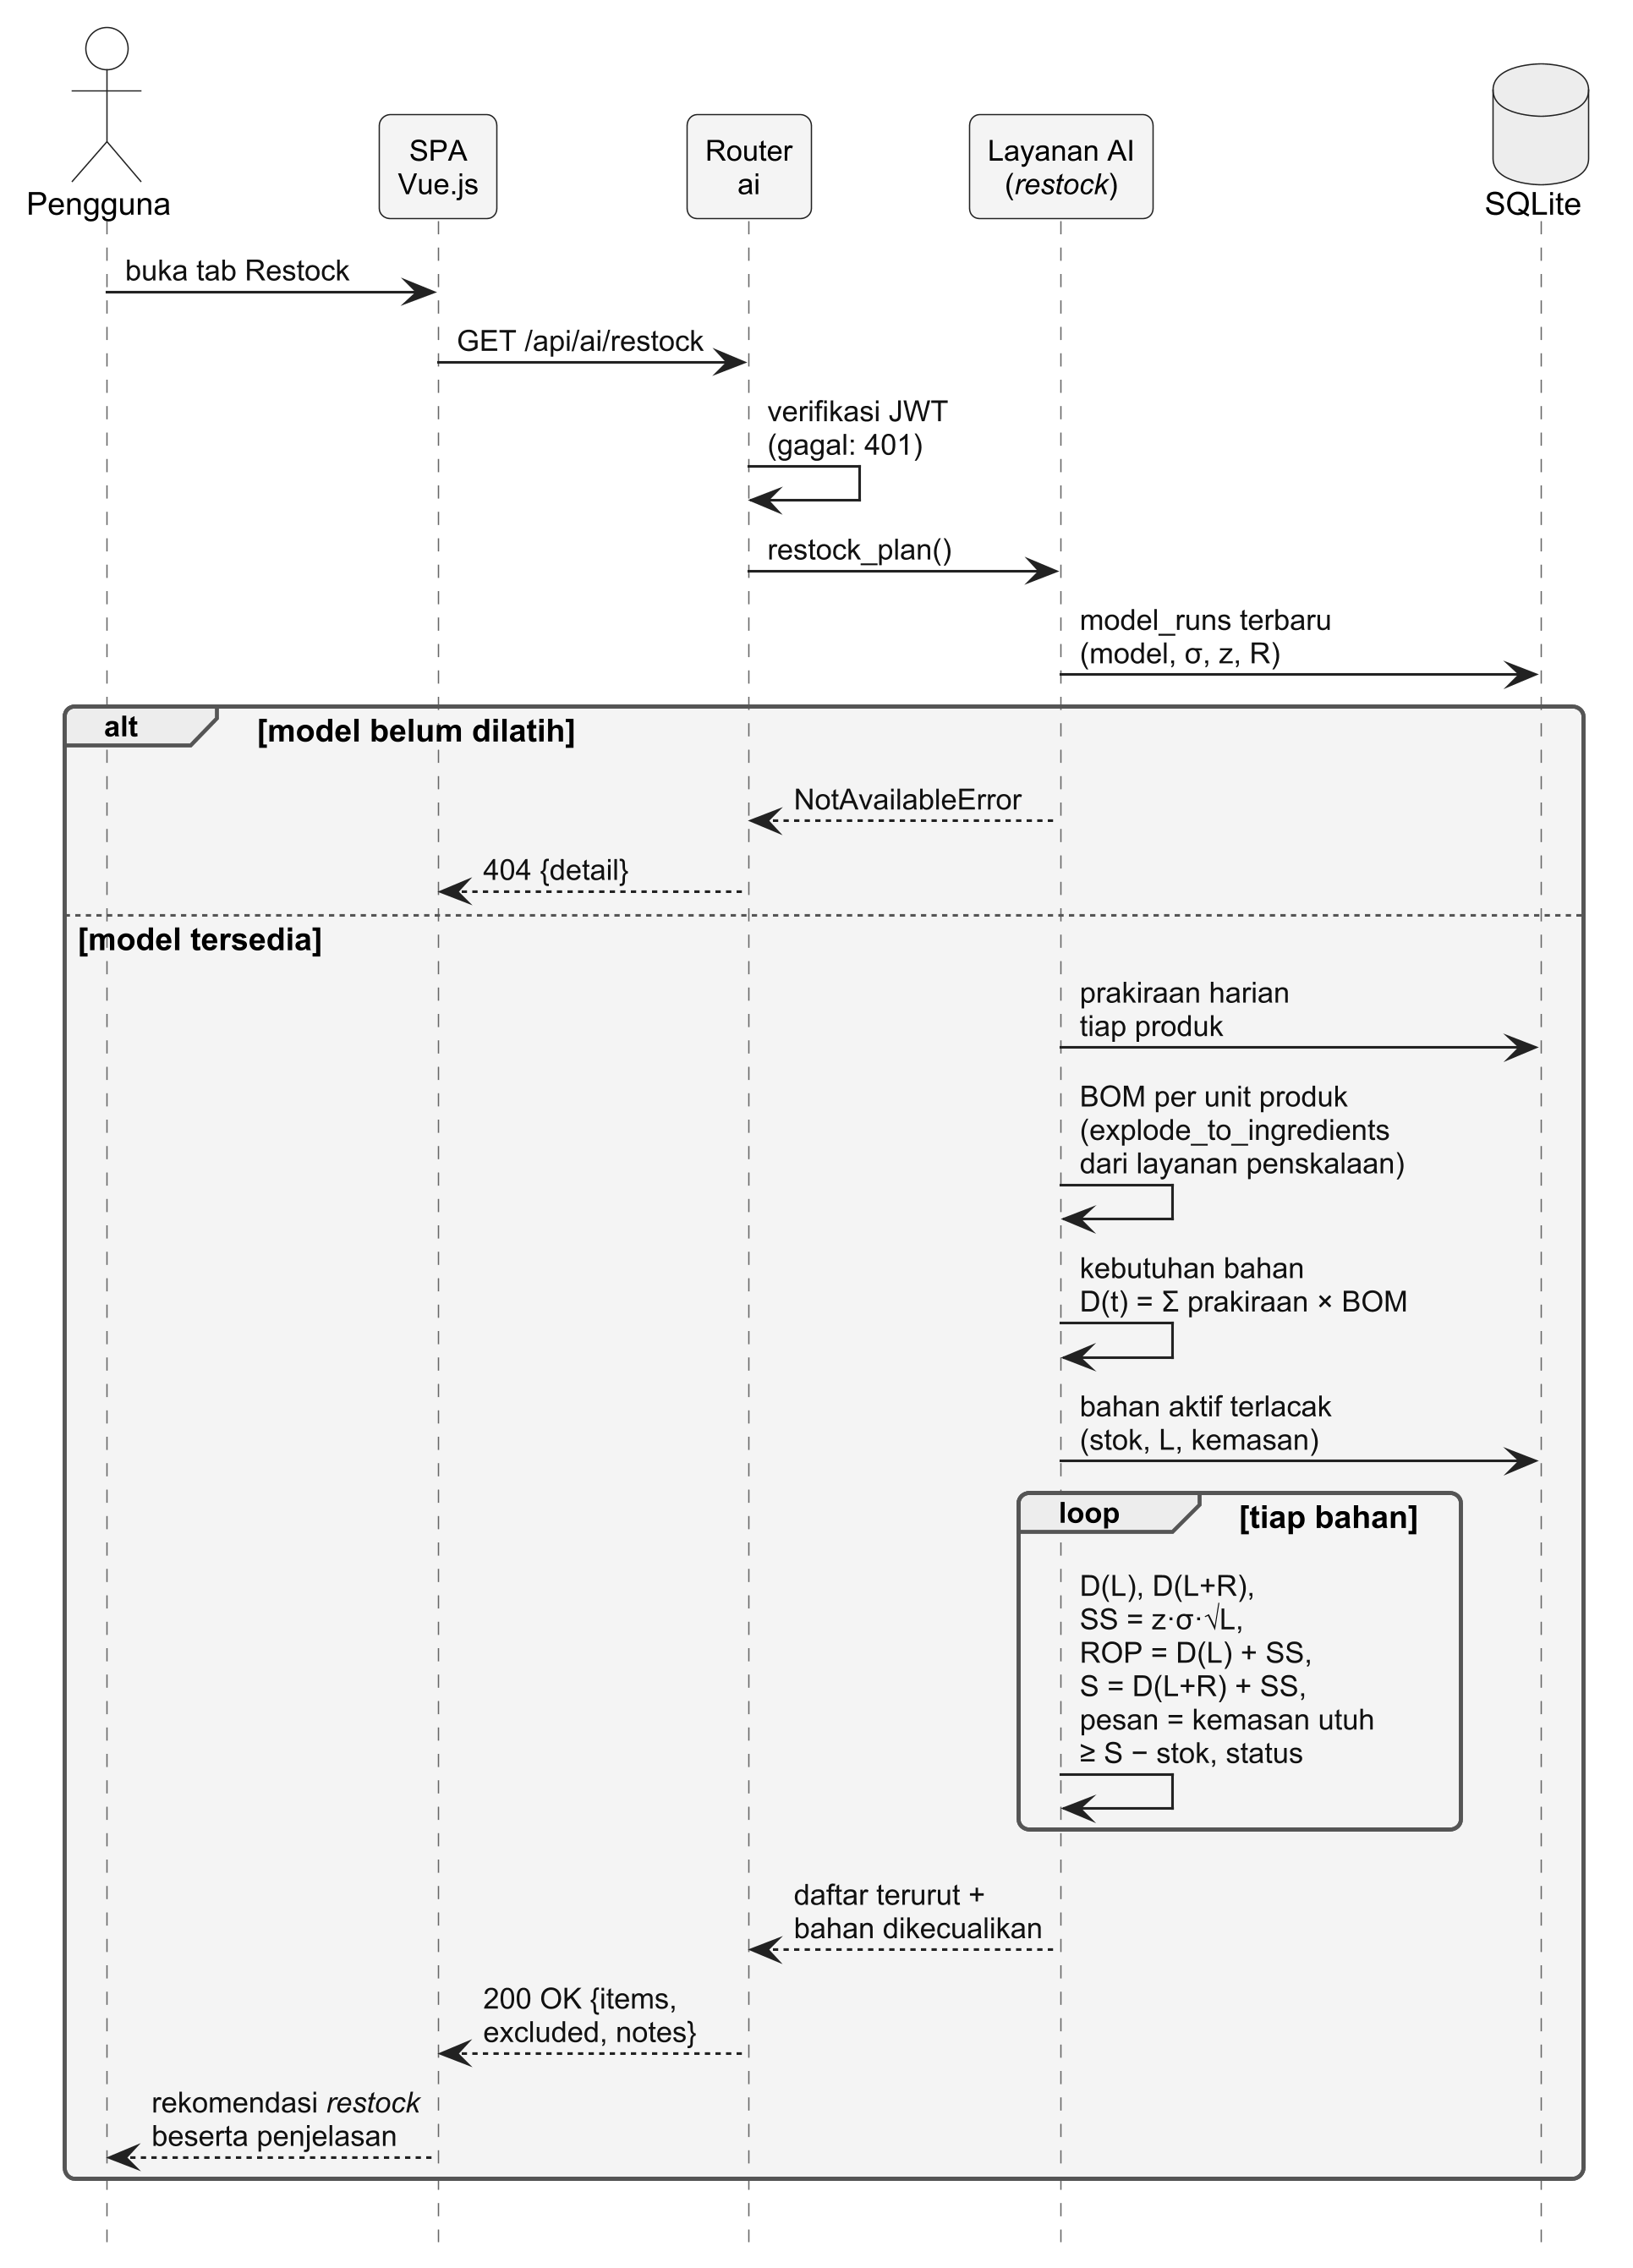
\includegraphics[width=.82\textwidth]{pic/sequence_restock.png}
\caption{Sekuens Peramalan dan Rekomendasi Pengisian Ulang}
\label{fig:sequence-restock}
\end{figure}

\subsection{Sistem Pakar Koreksi Seduh}

Sistem pakar menerima metode, dosis, massa air atau minuman, TDS bila tersedia, waktu, suhu, dan deskriptor rasa. Sistem menghitung rasio dan rendemen ekstraksi (EY) jika masukan cukup, lalu menolak kombinasi fisik yang tidak masuk akal. Basis pengetahuan JSON menyimpan kondisi, kesimpulan, prioritas, saran, dan sumber setiap aturan. Mesin inferensi \textit{forward chaining} memilih aturan cocok dengan prioritas tertinggi, menambahkan fakta baru, dan mengulang sampai tidak ada aturan yang dapat ditembakkan. Jejak aturan disajikan sebagai penjelasan diagnosis. Tabel~\ref{tab:aturan-pakar} meringkas kelompok aturan; ambang lengkap dan sumbernya disimpan dalam \texttt{app/backend/app/ai/kb/brew\_rules.json}.

\begin{table}[htbp]
\centering
\caption{Kelompok Aturan Sistem Pakar Koreksi Seduh}
\label{tab:aturan-pakar}
\begin{tabular}{p{.24\textwidth}p{.63\textwidth}}
\toprule
Kelompok & Tujuan aturan \\
\midrule
Validasi & Menolak input fisik yang tidak wajar atau satuan yang tidak sesuai. \\
Klasifikasi & Menentukan kekuatan dan tingkat ekstraksi dari TDS dan EY bila tersedia. \\
Standar resep & Membandingkan rasio, waktu, dan suhu terhadap resep atau standar literatur yang ditandai sumbernya. \\
Koreksi & Menyarankan perubahan gilingan, rasio, waktu, atau suhu sesuai gejala dan fakta yang tersedia. \\
Penjelasan & Menampilkan aturan yang ditembakkan dan alasan kondisi cocok. \\
\bottomrule
\end{tabular}
\end{table}

\subsection{Perancangan Asisten Barista AI}
\label{subsec:perancangan-asisten}

Asisten tanya-jawab memakai model bahasa yang dijalankan secara lokal melalui Ollama. Korpusnya dibangun dari resep, SOP, aturan sistem pakar, dan glosarium aplikasi; setiap potongan mempunyai pengenal serta tautan ke halaman asal. Pencarian BM25 mengambil potongan paling relevan dan menyediakan konteks yang dapat dikutip. Untuk pertanyaan praktis dengan maksud, entitas katalog, dan parameter yang cukup jelas, router deterministik terlebih dahulu menjalankan alat baca-saja yang memanggil layanan takaran, diagnosis, stok, atau pasangan menu; jawaban ini ditandai sebagai mode alat. Bila parameter untuk alat belum cukup, sistem dapat meminta rincian tanpa mengarang masukan. Pertanyaan lain diberikan kepada model bersama konteks yang ditemukan dan alat yang dapat dipanggil, dengan instruksi untuk menjawab dalam bahasa Indonesia, menyebut sumber, dan menyatakan ketidaktahuan bila fakta tidak tersedia. Pertanyaan di luar cakupan disaring sebelum model dipanggil. Saat model tidak tersedia atau penjaga jawaban menolak keluarannya, pencarian memberi cuplikan sumber dengan penanda mode pencarian yang jelas. Susunan ini adalah pipeline hibrida; hasil alat maupun penolakan dari aturan tidak boleh diatribusikan semata-mata kepada kemampuan Gemma 4.

Empat kondisi evaluasi dipisahkan: pencarian saja, model bahasa tanpa konteks, model dengan \textit{retrieval}, dan model dengan \textit{retrieval} serta alat. Tolok ukur tanya-jawab berbahasa Indonesia disiapkan dengan bantuan AI dari sumber resep, SOP, dan basis aturan; kutipan serta kunci jawaban diperiksa secara otomatis terhadap sumbernya, sedangkan jawaban numerik dihitung oleh layanan aplikasi pada waktu evaluasi. Metriknya mencakup ketepatan pencarian, ketepatan jawaban, pemilihan alat, penolakan pertanyaan di luar cakupan, angka tanpa dasar, latensi, dan jumlah peralihan ke mode pencarian. Tingkat halusinasi angka dihitung sebagai jumlah angka jawaban tanpa dukungan pertanyaan, sumber terambil, atau keluaran alat dibagi seluruh angka yang muncul dalam jawaban. H5 didukung hanya bila, pada model utama Gemma 4 E4B dan butir yang sama, akurasi jawaban kondisi RAG dengan alat lebih tinggi \emph{dan} tingkat halusinasi angkanya lebih rendah daripada kondisi tanpa konteks; Gemma 4 E2B menjadi pembanding tambahan. Butir serta penilaiannya belum mendapat peninjauan manual oleh peneliti maupun barista praktik, sehingga hasilnya bersifat tolok ukur internal dan belum dapat digeneralisasi ke penggunaan kedai.

Tolok ukur internal memuat 60 pertanyaan: 14 fakta resep, 12 prosedur/SOP, 10 perhitungan, delapan diagnosis seduh, enam stok, dan 10 di luar cakupan. Enam kondisi model berasal dari kombinasi tiga konfigurasi (tanpa konteks, RAG, serta RAG dengan alat) dan dua ukuran Gemma 4 (E4B dan E2B); pencarian BM25 tanpa model menjadi kondisi ketujuh. Evaluasi memakai suhu model nol dan \textit{seed} tetap 42, serta menyimpan jawaban mentah agar pemeriksaan skor dapat diulang tanpa memanggil model kembali.

Skor kondisi RAG dengan alat mencakup router deterministik, pemeriksaan luar cakupan, keluaran model, dan peralihan ke pencarian bila diperlukan. Karena itu, perbandingan H5 menilai sistem lengkap pada pertanyaan yang sama, bukan kemampuan model bahasa secara terisolasi. Selain akurasi isi yang menjadi ukuran utama H5, akurasi terverifikasi alat mensyaratkan nama alat dan argumen yang benar pada butir alat. Jumlah jawaban menurut mode alat, model, atau pencarian dilaporkan agar kontribusi masing-masing jalur dapat dibedakan. Akurasi khusus mode model dihitung hanya pada butir yang benar-benar dijawab model dan tidak dapat dibandingkan langsung sebagai kondisi pada keseluruhan 60 butir. Perutean alat disempurnakan setelah kegagalan pada butir tolok ukur awal terlihat; pengujian akhir pada butir yang sama adalah uji regresi internal, bukan estimasi generalisasi independen. Kueri tambahan di luar tolok ukur hanya berfungsi sebagai pemeriksaan cepat dan belum menjadi himpunan uji yang divalidasi manusia.

\section{\texorpdfstring{\textit{Dataset}}{Dataset}}
\label{sec:dataset}

Tabel~\ref{tab:dataset} memisahkan sumber pengembangan dari sumber validasi eksternal. Data mentah disimpan apa adanya di \texttt{dataset/raw}; salinan yang dinormalisasi berada di \texttt{dataset/processed}. Berkas \texttt{DATASHEET.md} pada setiap folder mencatat asal, lisensi, isi, dan keterbatasan. Hash berkas masukan tersimpan dalam hasil eksperimen sehingga perubahan data dapat dideteksi.

\begin{table}[htbp]
\centering
\caption{Sumber Data dan Perannya dalam Penelitian}
\label{tab:dataset}
\begin{tabular}{p{.23\textwidth}p{.22\textwidth}p{.17\textwidth}p{.25\textwidth}}
\toprule
Sumber & Sifat data & Jumlah utama & Penggunaan \\
\midrule
IBM Coffee Shop Sample Data & Sampel fiktif & 49.894 baris & Pengembangan pasangan menu. \\
Maven Coffee Shop Sales & Sampel fiktif & 149.116 baris & Pengembangan peramalan dan \textit{restock}. \\
The Bread Basket & Transaksi nyata; lisensi tidak jelas & 21.293 baris mentah & Validasi pasangan menu (E1). \\
ihelon Coffee Sales & Transaksi nyata; CC0 & 3.636 cangkir & Validasi peramalan dan \textit{restock} (E2--E3). \\
UC Davis/Cotter dan Batali & Eksperimen seduh nyata & 3.186 penilaian; 27 resep & Validasi sistem pakar (E4). \\
Menu Starbucks & Data menu terbitan publik & 7 minuman terpilih & Validasi aturan \textit{shot} per ukuran (E5). \\
\bottomrule
\end{tabular}
\end{table}

Produk publik dipetakan ke resep melalui berkas \texttt{product\_recipe\_map.json}. Tabel~\ref{tab:pemetaan-produk} memberi contoh yang menentukan kebutuhan bahan; pemetaan lengkap beserta asumsi ukuran terdapat pada berkas tersebut dan \texttt{ASSUMPTIONS.md}. Produk kemasan atau roti tanpa resep tidak dipaksakan menjadi minuman dan tidak ikut diuraikan menjadi bahan. Pemetaan ini adalah pendekatan untuk eksperimen, bukan catatan resep asli dari penerbit dataset.

\begin{table}[htbp]
\centering
\caption{Contoh Pemetaan Produk Dataset ke Resep}
\label{tab:pemetaan-produk}
\begin{tabular}{p{.38\textwidth}p{.42\textwidth}}
\toprule
Kelompok produk & Resep aplikasi atau perlakuan \\
\midrule
Latte, Cappuccino, Espresso & Caffè Latte, Cappuccino, Espresso Double. \\
Seduhan kopi tetes & V60 dengan biji yang dipetakan. \\
Cokelat panas, chai, teh & Resep tambahan Hot Chocolate, Chai Latte, Brewed Tea. \\
Sirup tambahan & Komponen bahan tambahan dengan takaran asumsi. \\
Roti dan barang kemasan & Produk akhir; tidak diuraikan menjadi bahan. \\
\bottomrule
\end{tabular}
\end{table}

\section{Rancangan Eksperimen dan Metrik Evaluasi}
\label{sec:rancangan-eksperimen}

Penskalaan diuji pada kombinasi resep jual, ukuran dan sajian yang sah, tingkat manis yang berlaku, tambahan \textit{shot}, jumlah cangkir, serta dosis V60 10--30~g. Tiga metode dijalankan pada pesanan yang sama. Tingkat pelanggaran dihitung untuk \textit{shot} pecahan, luapan lebih dari 5\%, kurang isi, penyimpangan rasio lebih dari 0,2, jumlah di luar batas, ketelitian takar yang tidak praktis, dan ketidaksesuaian jumlah batch. Pemeriksaan yang dijamin oleh bentuk algoritma ditandai sebagai hasil \textit{by construction}; nilai nol pada metrik demikian bukan bukti uji lapangan. Validasi E5 memakai jumlah \textit{shot} yang tersirat dari kafein menu sebagai pembanding eksternal dan membedakan aturan diskret dari tabel pengecualian yang mengambil angka menu itu sendiri.

Pasangan menu dibagi menurut waktu: periode awal untuk latih, bagian akhir latih untuk memilih ambang, dan periode terakhir untuk uji. Pada tiap keranjang uji dengan paling sedikit dua item berbeda, satu item disembunyikan bergantian. HR@1/3/5, Precision@5, MRR@5, cakupan kueri, dan cakupan katalog dibandingkan antara popularitas, peluang ko-okurensi, dan FP-Growth. Selang kepercayaan 95\% didapat dari \textit{bootstrap} keranjang, termasuk selisih berpasangan. Keranjang Maven didefinisikan secara heuristik dari toko, tanggal, dan waktu yang sama karena sumber itu tidak mempunyai nomor struk; hasilnya hanya analisis sekunder. E1 mengulang protokol pada nomor transaksi nyata Bread Basket.

Peramalan dinilai dengan delapan origin mingguan dan horizon tujuh hari. Pada setiap origin, model hanya boleh memakai pengamatan yang terjadi sampai origin tersebut. MAE dan RMSE menunjukkan besaran galat, WAPE mengukur galat absolut terhadap volume permintaan, MASE membandingkan dengan skala \textit{seasonal naive} pada data latih, dan bias menunjukkan arah kesalahan; bias positif berarti ramalan terlalu tinggi. Selain pada produk, ramalan diuraikan melalui BOM menjadi satuan bahan. E2 menguji model yang dipilih pada Maven tanpa memilih ulang model memakai jendela uji ihelon, baik per minuman maupun pada total harian.

Simulasi \textit{restock} memutar ulang 56 hari terakhir permintaan bahan. Kebijakan ramalan tingkat sasaran dibandingkan dengan ROP statis dan tingkat persediaan par; varian pembanding mengendalikan struktur pemesanan dan pilihan model ramalan. Ukuran utama adalah \textit{fill rate}, jumlah hari kehabisan stok, rata-rata stok dalam hari permintaan, dan frekuensi pesanan. Setiap kebijakan menerima stok awal dan asumsi pasokan yang sama. E3 mengulang pada permintaan ihelon yang dipetakan ke tiga bahan demo; keputusan H4 hanya berlaku pada perbandingan kebijakan utama dan ROP statis, bukan pada klaim bahwa model ramalannya terbaik.

Sistem pakar dinilai dari reproduksi EY, kesesuaian arah klasifikasi kekuatan terhadap penilaian konsumen, dan arah koreksi terhadap perubahan parameter pada resep eksperimen. Angka kesukaan konsumen juga dibandingkan di dalam dan di luar kotak \textit{Golden Cup}; kotak tersebut tidak didefinisikan sebagai label kesukaan yang pasti. Pengujian ini membedakan ketepatan perhitungan dari kecocokan preferensi inderawi. Uji asisten lokal mengikuti rancangan pada Subbab~\ref{subsec:perancangan-asisten} dan dilaporkan hanya setelah berkas hasilnya tersedia.

\section{Rancangan Pengujian}
\label{sec:rancangan-pengujian}

Pengujian unit memeriksa aturan penskalaan, buku besar stok, sistem pakar, dan pembantu model AI. Pengujian API memeriksa respons berhasil, nilai batas, masukan tidak sah, serta pembatasan peran. Pengujian \textit{end-to-end} menjalankan alur masuk, resep, kalkulator, produksi, SOP, stok, rekomendasi, dan tampilan ponsel pada hasil \textit{build} yang disajikan server. Basis data uji antarmuka merupakan salinan agar produksi uji tidak mengubah basis data demo. Kasus uji dan hasil aktual ditulis otomatis ke \texttt{app/results/tests}.

Kinerja API diukur setelah pemanasan dengan permintaan berulang pada komputer pengembangan; hasil ini merupakan latensi lingkungan uji, bukan jaminan pada semua perangkat. Audit Lighthouse dilakukan pada halaman masuk publik untuk desktop dan ponsel. Uji penerimaan pengguna dirancang sebagai penyelesaian tugas barista dan kuesioner \textit{System Usability Scale} (SUS) 10 butir. Pelaksanaan bersama pengguna kedai dan nilainya belum tersedia; penelitian ini tidak mengisi skor atau testimoni yang belum dikumpulkan.

\section{Jadwal Penelitian}
\label{sec:jadwal}

Jadwal kegiatan disusun menurut ketergantungan keluaran, seperti pada Tabel~\ref{tab:jadwal}. Tanggal pelaksanaan formal dan sesi uji penerimaan dengan kedai mitra perlu disepakati setelah mitra penelitian dan pembimbing dikonfirmasi. Karena itu, tabel ini menyatakan urutan kerja, bukan tanggal kegiatan yang belum dapat diverifikasi.

\begin{table}[htbp]
\centering
\caption{Urutan Kegiatan Penelitian}
\label{tab:jadwal}
\begin{tabular}{p{.09\textwidth}p{.24\textwidth}p{.50\textwidth}}
\toprule
Urutan & Kegiatan & Keluaran \\
\midrule
1 & Analisis kebutuhan dan sumber & Kebutuhan peran, resep arahan, dan lembar data dataset. \\
2 & Perancangan & Skema data, antarmuka, aturan penskalaan, dan protokol evaluasi. \\
3 & Implementasi bertahap & API, antarmuka, basis pengetahuan, dan skrip model. \\
4 & Pengujian dan evaluasi & Kasus uji, metrik algoritma, dan validasi eksternal. \\
5 & UAT dan penyusunan akhir & Hasil tugas pengguna dan SUS setelah sesi nyata dilaksanakan. \\
\bottomrule
\end{tabular}
\end{table}
